\subsection{Case Report Identification Performance}
\label{sec:results_case_identification}

\begin{table}[t!]
\footnotesize
\centering
\caption{\rebuttal{Case-report identification performance by diagnosis and in aggregate on the manually reviewed 100-document evaluation set. Recall is calculated with respect to confirmed single-patient case reports within this evaluation set.}}
\label{tab:case_report_identification}
% \begin{adjustbox}{max width=0.95\textwidth}
\begin{tabular}{llcccc}
\toprule
Subset & Diagnosis & Precision & Recall & Accuracy & F1 Score \\
\midrule
\multirow{6}{*}{PubMed metadata} 
    & Atrial Fibrillation & 0.84 & 0.94 & 0.80 & 0.89 \\
    & COVID-19            & 0.94 & 0.89 & 0.85 & 0.92 \\
    & Diabetes            & 0.85 & 1.00 & 0.85 & 0.92 \\
    & Hypertension        & 1.00 & 1.00 & 1.00 & 1.00 \\
    & Sepsis              & 0.95 & 0.95 & 0.90 & 0.95 \\
\cmidrule(lr){2-6}
    & \textbf{All Diagnoses} & \text{0.92} & \textbf{0.96} & \text{0.88} & \text{0.94} \\
\midrule
\multirow{6}{*}{LLM-Pipeline}
    & Atrial Fibrillation & 1.00 & 1.00 & 1.00 & 1.00 \\
    & COVID-19            & 1.00 & 0.89 & 0.90 & 0.94 \\
    & Diabetes            & 1.00 & 0.94 & 0.95 & 0.97 \\
    & Hypertension        & 1.00 & 0.95 & 0.95 & 0.97 \\
    & Sepsis              & 1.00 & 1.00 & 1.00 & 1.00 \\
\cmidrule(lr){2-6}
    & \textbf{All Diagnoses} & \textbf{1.00} & \textbf{0.96} & \textbf{0.96} & \textbf{0.98} \\
\bottomrule
\end{tabular}
% \end{adjustbox}
\vspace{-5mm}
\end{table}



% \begin{table}[!ht]
%     \footnotesize
%     \centering
%     \caption{Case report identification performance per diagnosis}
%     \label{tab:diagnosis_results}
%     \begin{tabular}{l l c c c c c}
%         \hline
%         Subset & Diagnosis & Sensitivity & Specificity & Accuracy & Precision & F1 Score \\
%         \hline
%         PubMed MetaData  & Atrial Fibrillation & 0.94 & 0.00 & 0.80 & 0.84 & 0.89 \\
%         LLM-Pipeline     & Atrial Fibrillation & 1.00 & 1.00 & 1.00 & 1.00 & 1.00 \\
%         \hline
%         PubMed MetaData  & COVID-19           & 0.89 & 0.00 & 0.85 & 0.94 & 0.92 \\
%         LLM-Pipeline     & COVID-19           & 0.89 & 1.00 & 0.90 & 1.00 & 0.94 \\
%         \hline
%         PubMed MetaData  & Diabetes           & 1.00 & 0.00 & 0.85 & 0.85 & 0.92 \\
%         LLM-Pipeline     & Diabetes           & 0.94 & 1.00 & 0.95 & 1.00 & 0.97 \\
%         \hline
%         PubMed MetaData  & Hypertension       & 1.00 & 0.00 & 1.00 & 1.00 & 1.00 \\
%         LLM-Pipeline     & Hypertension       & 0.95 & 0.00 & 0.95 & 1.00 & 0.97 \\
%         \hline
%         PubMed MetaData  & Sepsis             & 0.95 & 0.00 & 0.90 & 0.95 & 0.95 \\
%         LLM-Pipeline     & Sepsis             & 1.00 & 1.00 & 1.00 & 1.00 & 1.00 \\
%         \hline
%     \end{tabular}
% \end{table}

% \begin{table}[!ht]
%     \footnotesize
%     \centering
%     \caption{Aggregated case report identification performance across all diagnoses}
%     \label{tab:aggregated_results}
%     \begin{tabular}{l c c c c c}
%         \hline
%         Subset & Sensitivity & Specificity & Accuracy & Precision & F1 Score \\
%         \hline
%         PubMed MetaData  & \textbf{0.96} & 0.00 & 0.88 & 0.92 & 0.94 \\
%         LLM-Pipeline     & \textbf{0.96} & \textbf{1.00} & \textbf{0.96} & \textbf{1.00} & \textbf{0.98} \\
%         \hline
%     \end{tabular}
% \end{table}

Our evaluation of case report identification methods compared our LLM-Pipeline approach against PubMed's metadata-based filtering across five different diagnoses: Diabetes, Sepsis, Hypertension, COVID-19, and Atrial Fibrillation. 
Using clinician-assigned labels as ground truth, we computed precision, recall, accuracy, and F1 score for each approach.

The LLM-Pipeline approach demonstrates superior performance with perfect precision (1.00) across all diagnostic categories and also aggregated across all diagnoses (Table~\ref{tab:case_report_identification}), indicating that when our pipeline identifies a document as a single-patient case report, it is always correct \textcolor{red}{Jeremy: modify to not overstate}. In contrast, the PubMed MetaData approach shows more variable precision, ranging from 0.84 for Atrial Fibrillation to 1.00 for Hypertension, with an overall precision of 0.92.

Both methods achieve similar recall (0.96), indicating comparable success in identifying true case reports.
However, the LLM-Pipeline attains higher overall accuracy (0.96 vs. 0.88), reflecting its superior ability to distinguish both true positives and true negatives. This accuracy gain is largely due to the LLM-Pipeline’s effectiveness in excluding non-single-patient reports, which the PubMed MetaData approach often misclassifies.

Examining performance by diagnostic category reveals that both approaches perform best on Sepsis and Hypertension cases, while showing more variability with Atrial Fibrillation, COVID-19, and Diabetes reports. The LLM-Pipeline maintains consistently high performance across all categories, with F1 scores ranging from 0.94 to 1.00. These findings highlight the significant improvements in precision and overall classification quality offered by our LLM-Pipeline approach for case report identification, ensuring that the PMOA-TTS corpus contains high-quality, single-patient case reports with minimal contamination from multi-patient or non-case report documents.


%%%%%%%%%%%%%%%%%%%%%%%%%%%%%%%%%%%%%%%%%%%%%%%%%
%%%%%%%%%%%%%%%%%%%%%%%%%%%%%%%%%%%%%%%%%%%%%%%%%

\subsection{Evaluation of Clinical Textual Time Series Quality}

We assessed the quality of the extracted textual time series using 200 manually annotated case reports as reference. 
Each large language model (LLM) was evaluated across five independent runs to account for variability in annotation consistency. 
Table~\ref{tab:model_comparison} summarizes the results for \texttt{DeepSeek-R1}, \texttt{DeepSeek-V3-0324}, \texttt{LLaMA 3.3 70B}, \texttt{OpenAI O1}, \texttt{OpenAI O3}, \texttt{OpenAI O4-mini}, and \texttt{OpenAI GPT5}, comparing performance across three metrics: Match Rate, Concordance, and AULTC. 
Among these models, \texttt{OpenAI GPT5} achieved the highest mean Match Rate (0.47 $\pm$ 0.005), while \texttt{OpenAI O3} achieved the highest Concordance (0.891 $\pm$ 0.006), and \texttt{OpenAI O4-mini} achieved the highest AULTC (0.748 $\pm$ 0.003). 
The standard deviations across runs were generally low, indicating consistent performance within each model across repetitions.
The standard deviations across runs were generally low, indicating consistent performance within each model across repetitions.

% We evaluated the quality of extracted textual time series using the manually annotated subset as ground truth, comparing seven LLM variants: \texttt{DeepSeek-R1}, 
% % DeepSeek-R1-UD-IQ1, 
% \texttt{DeepSeek-V3-0324}, \texttt{LLaMA 3.3 70B}, \texttt{OpenAI O1}, \texttt{OpenAI O3}, \texttt{OpenAI O4-mini}, and \texttt{OpenAI GPT5}. 
%A comparison of different LLM annotations and sensitivity to different prompt strategies can be found in Appendices \ref{apd:example_annotations} and \ref{apd:prompt_ablation} respectively. 

\begin{table}[h!]
\centering
\caption{Comparison of models on Match Rate, Concordance, and AULTC with respect to 200 manually annotated case reports across 5 different runs for each model.}
\label{tab:model_comparison}
\begin{tabular}{lccc}
\hline
\textbf{Model} & \textbf{Match Rate} & \textbf{Concordance} & \textbf{AULTC} \\
\hline
\texttt{LLaMA 3.3 70B}       & 0.675 $\pm$ 0.003 & 0.835 $\pm$ 0.003 & 0.717 $\pm$ 0.001 \\
\texttt{DeepSeek-R1}         & 0.746 $\pm$ 0.008 & 0.785 $\pm$ 0.010 & 0.726 $\pm$ 0.003 \\
\texttt{DeepSeek-V3-0324}    & 0.761 $\pm$ 0.004 & 0.791 $\pm$ 0.005 & 0.728 $\pm$ 0.002 \\
\texttt{OpenAI GPT5}         & \textbf{0.847 $\pm$ 0.005} & 0.883 $\pm$ 0.002 & 0.719 $\pm$ 0.001 \\
\texttt{OpenAI O4-mini}      & 0.750 $\pm$ 0.019 & 0.842 $\pm$ 0.008 & \textbf{0.748 $\pm$ 0.003} \\
\texttt{OpenAI O3}           & 0.736 $\pm$ 0.003 & \textbf{0.891 $\pm$ 0.006} & 0.735 $\pm$ 0.003 \\
\texttt{OpenAI O1}           & 0.638 $\pm$ 0.007 & 0.880 $\pm$ 0.003 & 0.730 $\pm$ 0.001 \\
\hline
\end{tabular}
\end{table}

To quantify uncertainty from a complementary perspective, we also performed a bootstrap analysis based on a single run per model (Table~\ref{tab:bootstrap_intervals}). 
In this setup, 200 samples were resampled with replacement to estimate 95\% confidence intervals for each metric. 
The bootstrapped intervals provide an estimate of variability arising from the sampling of annotated case reports rather than from repeated model runs. 
Together, these two evaluations capture variation both across model executions and across sampled annotations, providing a comprehensive view of model performance stability.

\begin{table}[ht!]
\centering
\caption{Bootstrap 95\% confidence intervals for Match Rate, Concordance, and AULTC across models evaluated on the 200 manually annotated case reports.}
\label{tab:bootstrap_intervals}
\begin{tabular}{lccc}
\hline
\textbf{Model} & \textbf{Match Rate (95\% CI)} & \textbf{Concordance (95\% CI)} & \textbf{AULTC (95\% CI)} \\
\hline
\texttt{LLaMA 3.3 70B}      & [0.6420, 0.7176] & [0.8333, 0.8611] & [0.7010, 0.7540] \\
\texttt{DeepSeek-R1}        & [0.6944, 0.7733] & [0.7825, 0.8175] & [0.7080, 0.7515] \\
\texttt{DeepSeek-V3-0324}   & [0.7269, 0.7905] & [0.7923, 0.8214] & [0.7178, 0.7581] \\
\texttt{OpenAI GPT5}        & [0.8047, 0.8661] & [0.8815, 0.8986] & [0.7056, 0.7498] \\
\texttt{OpenAI O4-mini}     & [0.6921, 0.7672] & [0.8263, 0.8515] & [0.7320, 0.7696] \\
\texttt{OpenAI O3}          & [0.6986, 0.7654] & [0.8879, 0.9062] & [0.7278, 0.7645] \\
\texttt{OpenAI O1}          & [0.5990, 0.6772] & [0.8719, 0.8952] & [0.7163, 0.7550] \\
\hline
\end{tabular}
\end{table}

% \begin{itemize}
%     \item \textcolor{red}{Figure is too big. Push it to Appendix and have a table in main? (like T2S2 paper)}
% \end{itemize}


\subsubsection{Text Event Match Performance}
%\textbf{Text Event Match Performance.} 
Figure~\ref{fig:tts_evaluation} (left) shows the cumulative density of cosine distances between model-generated and reference event descriptions. A threshold of 0.1 (vertical line) defines a successful match. \texttt{DeepSeek-R1} (black) and its quantized variant \texttt{DeepSeek-R1-UD-IQ1} (orange) outperform other models, with ~80\% of aligned events falling below the threshold. \texttt{DeepSeek-V3-0324} (light blue) and \texttt{O4-mini} (red) form a second tier, while \texttt{LLaMA 3.3 70B} (green), \texttt{O1} (light yellow), and \texttt{O3} (blue) show more dispersed distributions, with only 70\% of events below the threshold. These analyses highlights clear differences in how well models generate event descriptions that align semantically with expert annotations. The strong performance of \texttt{DeepSeek-R1} and its quantized variant indicates their enhanced ability to model clinical language patterns found in case reports.


\subsubsection{Temporal Ordering Performance}
%\textbf{Temporal Ordering Performance.} 
Using the cosine distance threshold to identify matched events, we assessed temporal ordering accuracy via the concordance index (c-index).
As shown in Figure~\ref{fig:tts_evaluation} (right), \texttt{LLaMA 3.3 70B} achieves the highest median c-index (0.96), with \texttt{DeepSeek-V3-0324} and \texttt{DeepSeek-R1} following closely.

% \begin{figure}[!tbp]
% \centering
%     \begin{minipage}[t]{0.242\textwidth}
%     \centering
%     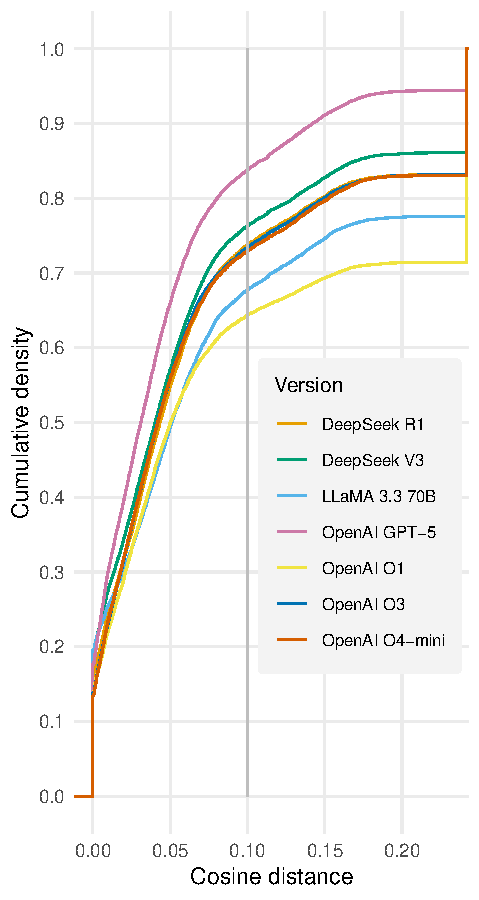
\includegraphics[page=1, width=\linewidth]{Plots_tables/pmoa_updated_man_figs.pdf}
%     \end{minipage}
%     \hfill
%     \begin{minipage}[t]{0.242\textwidth}
%     \centering
%     \includegraphics[page=2, width=\linewidth]{Plots_tables/pmoa_updated_man_figs.pdf}
%     \end{minipage}
%     \hfill
%     \begin{minipage}[t]{0.242\textwidth}
%     \centering
%     \includegraphics[page=3, width=\linewidth]{Plots_tables/pmoa_updated_man_figs.pdf}
%     \end{minipage}
%     \hfill
%     \begin{minipage}[t]{0.242\textwidth}
%     \centering
%     \includegraphics[page=4, width=\linewidth]{Plots_tables/pmoa_updated_man_figs.pdf}
%     \end{minipage}
%     \caption{Comparison of different LLM for extracting temporal clinical events from case reports. From left to right: (\textbf{A}) event match cumulative distribution function, (\textbf{B}) concordance box plots, (\textbf{C}) time discrepancy from manual annotation timestamps among matched events (overall), and (\textbf{D}) time discrepancy disaggregated by clinician annotator timestamp (time from presentation). 
%     %\textcolor{red}{Have same figure for LAPJV?}
%     }
%     \label{fig:tts_evaluation}
%     \vspace{-10pt}
% \end{figure}



\begin{figure}[!tbp]
\centering

% First row: panels A and B
\begin{minipage}[t]{0.49\linewidth}
    \centering
    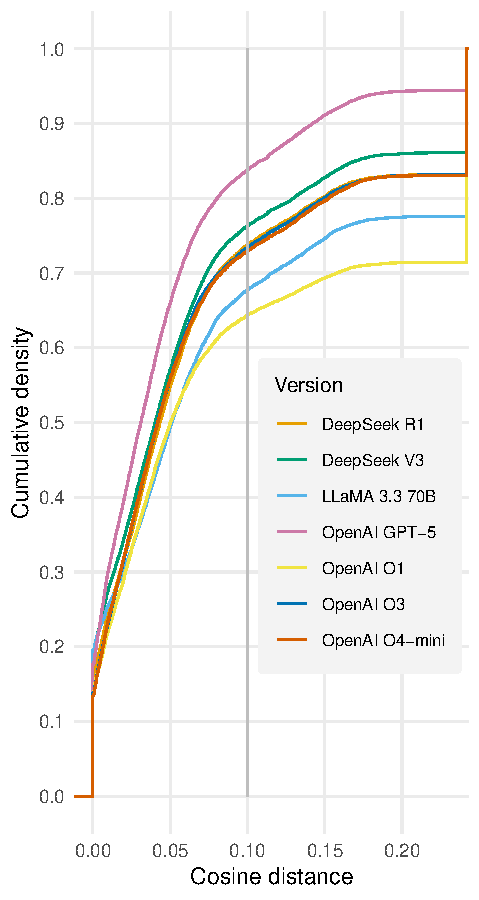
\includegraphics[
        page=1,
        width=0.8\linewidth
    ]{Plots_tables/pmoa_updated_man_figs.pdf}
\end{minipage}
\hfill
\begin{minipage}[t]{0.49\linewidth}
    \centering
    \includegraphics[
        page=2,
        width=0.8\linewidth
    ]{Plots_tables/pmoa_updated_man_figs.pdf}
\end{minipage}

\par\medskip

% Second row: panels C and D
\begin{minipage}[t]{0.49\linewidth}
    \centering
    \includegraphics[
        page=3,
        width=0.8\linewidth
    ]{Plots_tables/pmoa_updated_man_figs.pdf}
\end{minipage}
\hfill
\begin{minipage}[t]{0.49\linewidth}
    \centering
    \includegraphics[
        page=4,
        width=0.8\linewidth
    ]{Plots_tables/pmoa_updated_man_figs.pdf}
\end{minipage}

\caption{
Comparison of different LLMs for extracting temporal clinical events
from case reports:
(\textbf{A}) cumulative distribution of event-matching cosine distances;
(\textbf{B}) temporal-concordance box plots;
(\textbf{C}) timestamp discrepancies between model-generated and manual
annotations among semantically matched events; and
(\textbf{D}) timestamp discrepancies stratified by the clinician-annotated
time relative to presentation.
}
\label{fig:tts_evaluation}
\vspace{-10pt}
\end{figure}

The relationship between event matching and concordance evaluation is important to consider. Models applying stricter matching thresholds may appear to perform better on concordance by evaluating only the most confidently matched events. In contrast, models matching a broader set of events—including more ambiguous cases—encounter a more difficult ordering task. \texttt{LLaMA 3.3 70B}’s strong performance in temporal ordering is notable given its lower match rate, suggesting it effectively captures relative timing even when its textual matches are less precise.
\Cref{sec:choosing_match_threshold} discusses how adjusting the event match threshold allows tuning the balance between match coverage and ordering accuracy.

\subsubsection{Time Discrepancy Analysis}
%\textbf{Time Discrepancy Analysis.} 
Figure~\ref{fig:tts_evaluation} (left) displays the cumulative probability distribution of time differences (log-scaled) between predicted and reference timestamps, illustrating each model’s timestamping accuracy.
\texttt{DeepSeek-R1} (black line) shows the steepest curve, indicating that a higher proportion of its predictions are temporally close to the reference points. In contrast, \texttt{LLaMA 3.3 70B} (green line) produces a flatter curve, reflecting greater variation and lower precision in absolute time prediction. The right panel in Figure \ref{fig:tts_evaluation} breaks down performance across time intervals—presentation, 1 hour, 1 day, 1 week, 1 year, and beyond. All models perform well for events near the presentation time, but their accuracy declines as the temporal distance increases. \texttt{DeepSeek} models consistently show stronger performance across intervals, whereas \texttt{LLaMA 3.3 70B} exhibits more noticeable degradation for distant events.

Taken together, this analysis highlights a key distinction: while \texttt{LLaMA 3.3 70B} is more effective at predicting relative event order (concordance), \texttt{DeepSeek models}---particularly \texttt{DeepSeek-R1}---are better at assigning precise timestamps, even for events far from the reference point.

%%%%%%%%%%%%%%%%%%%%%%%%%%%%%%%%%%%%%

\subsubsection{Varying the Event Match Distance Threshold} \textcolor{red}{Move to Appendix with figures?}
\label{sec:choosing_match_threshold}

We also discuss how adjusting the event match threshold allows tuning the balance between match coverage and ordering accuracy. By varying the event match distance threshold, we obtain different performance characteristics for event match rate, event concordance, and temporal discrepancy (AULTC).  We choose a cosine similarity of 0.1 based on manual review of \texttt{Llama 3.3 70B Instruct} and \texttt{O1} annotations.  Plotting the event match rate versus temporal performance characteristic (concordance and AULTC) when varying the threshold from 0.01 to 0.25, we obtain performance tradeoffs in Figure \ref{fig:threshold_temporal_tradeoff}.

\begin{figure}
    \centering
    % \begin{minipage}{0.45\textwidth}
        % \centering
        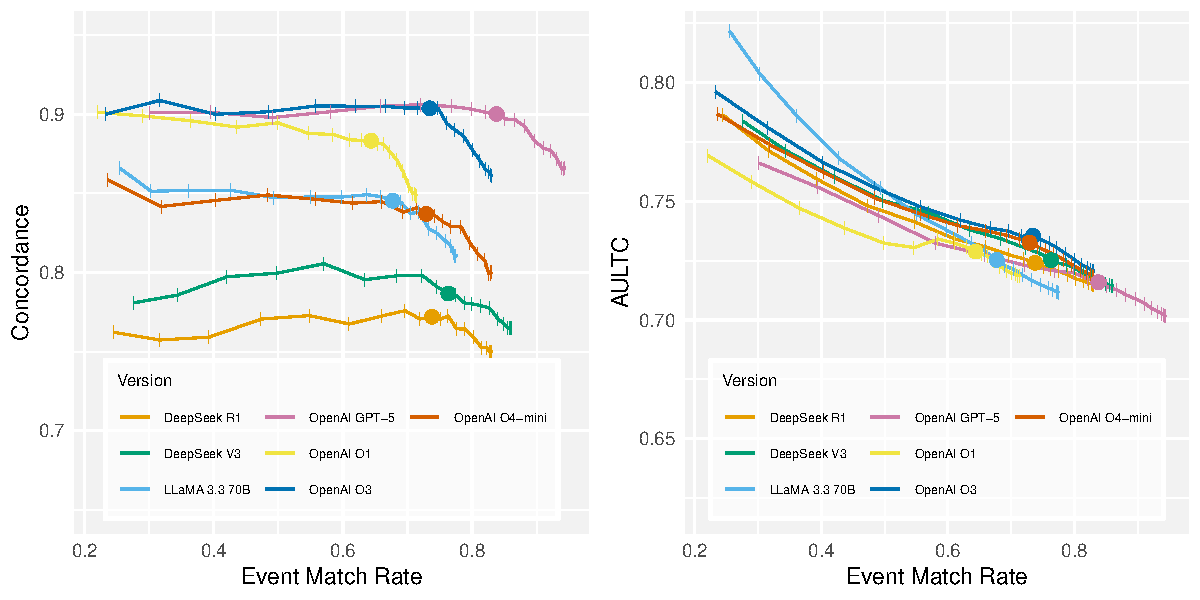
\includegraphics[width=\linewidth]{Plots_tables/event_match_vs_metrics_updated.pdf}
        % \caption{}
    % \end{minipage}
    % \hfill
    \caption{\textbf{Left:} Concordance by event match rate. Solid circle ($\bullet$) represents threshold of 0.1, with ticks (|) indicating 0.01 increments of the threshold in [0.01, 0.50]. \textbf{Right:} AULTC by event match rate.
    % \textcolor{red}{Remove \texttt{DSR1-quantized} and replace with \texttt{GPT5}. Rerun on 200?}
    }
    \label{fig:threshold_temporal_tradeoff}
\end{figure}


% \begin{figure}
%     \centering
%     \begin{minipage}{0.45\textwidth}
%         \centering
%         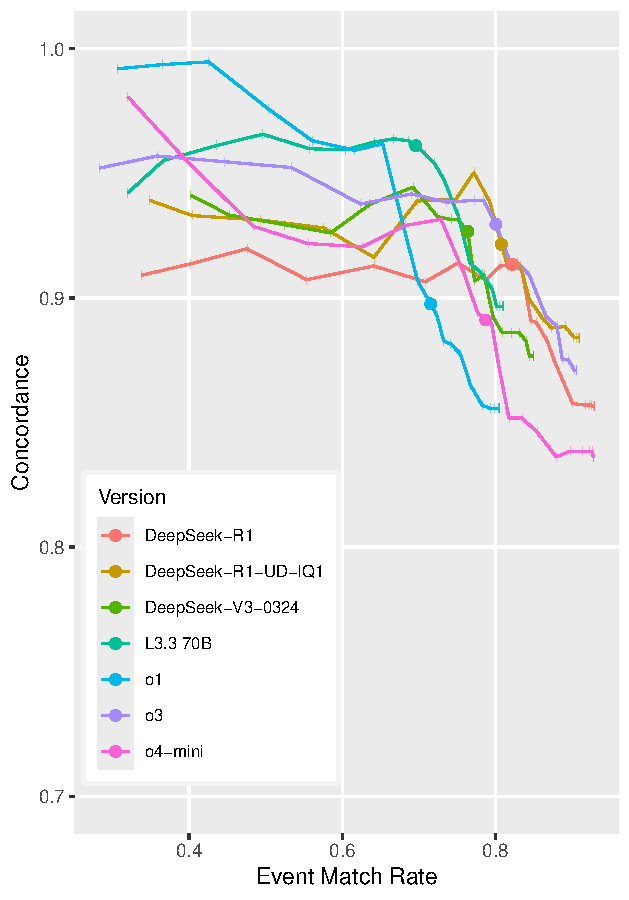
\includegraphics[width=\linewidth]{Plots_tables/match_threshold_concordance_plot.pdf}
%         % \caption{}
%     \end{minipage}
%     % \hfill
%     \begin{minipage}{0.45\textwidth}
%         \centering
%         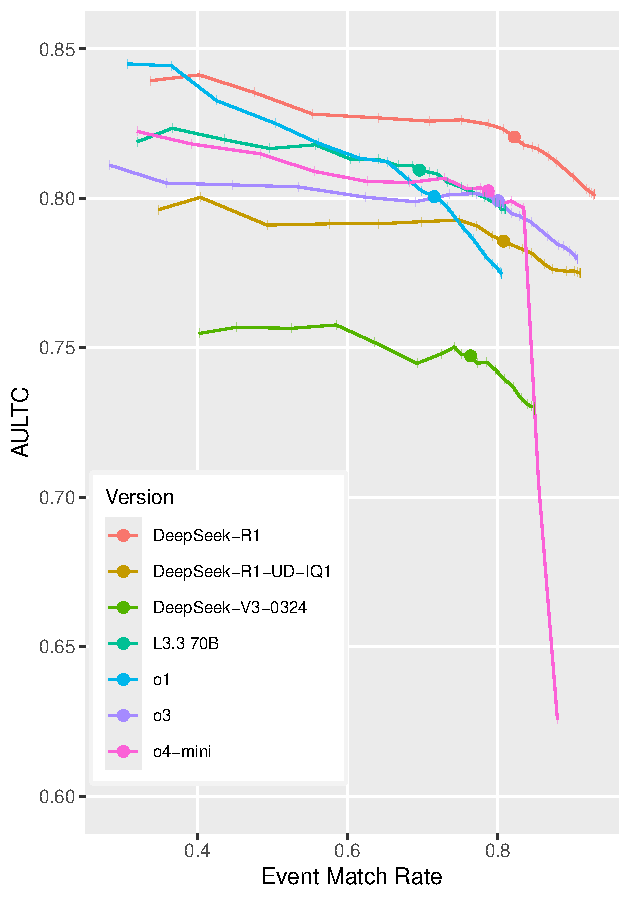
\includegraphics[width=\linewidth]{Plots_tables/match_threshold_plot.pdf}
%         % \caption{}
%     \end{minipage}
%     \caption{\textbf{Left:} Concordance by event match rate. Solid circle ($\bullet$) represents threshold of 0.1, with ticks (|) indicating 0.01 increments of the threshold in [0.01, 0.25]. \textbf{Right:} AULTC by event match rate.
%     \textcolor{red}{Remove \texttt{DSR1-quantized} and replace with \texttt{GPT5}. Rerun on 200?}
%     }
%     \label{fig:threshold_temporal_tradeoff}
% \end{figure}

%%%%%%%%%%%%%%%%%%%%%%%%%%%%%%%%%%%%%%%%%

\subsubsection{Annotation quality with prompt variation} \textcolor{red}{Move to Appendix?}

Figure \ref{fig:prompt_ablation} presents sensitivity analyses for different prompt strategies in extracting structured time series from clinical narratives. Each ablation tests the effect of removing specific instructional components or adding structured extraction requirements. We evaluate event-level semantic similarity, timestamp accuracy, and temporal concordance across matched events. 

% \noindent\textcolor{red}{Figure is too large, pushed it to Appendix. Have a table in main like T2S2 paper?}

\subsubsection{Sensitivity to Parts of the LLM Prompt Being Changed} \textcolor{red}{Move to Appendix?}
% % \section{Sensitivity to Parts of the LLM Prompt Being Changed} \textcolor{red}{Move to Appendix?}

% We slightly modified the prompt from the preceding section to check for sensitivity to specific parts of the LLM prompt being removed or modified.
% % For sensitivity analyses with respect to the quality of different prompt strategies for extracting textual time-series (\texttt{DeepSeek R1}) from PMOA case reports, we omitted selected sections of the LLM query prompt
% % (see Appendix \ref{apd:extraction_prompt} for the full prompt).
% This led to the following variants:
% \begin{enumerate}
%     \item \textbf{No changes}: Original LLM query prompt. % for \texttt{DeepSeek-R1}.
    
%     \item \textbf{No role:} Remove the initial sentence \texttt{"You are a physician."}.
    
%     \item \textbf{Zero-shot prompting:} Remove the example case report and textual time-series from the prompt. \\
%     %\item \textbf{No conjunction expansion:} 
%     \textcolor{teal}{\texttt{An 18-year-old male was admitted to ..}}\\
%     "Let's find the locations of event in the case report, it shows that ... then the output should look like:"\\
%     \texttt{18 years old | 0 \\
%     male | 0 \\
%     ..}

%     \item \textbf{No conjunction expansion:} Remove the following sentence from the prompt: \texttt{"Separate conjunctive phrases into its component events and assign them the same timestamp (for example, separation of ‘fever and rash’ into 2 events: ‘fever’ and ‘rash’)"}
    
%     \item \textbf{Interval:} A query was added to the prompt for extracting the time interval (start and end time of clinical events). The original prompt’s instructions and few-shot examples were modified accordingly. 
    
%     \item \textbf{Interval + Type:} A query was added to the prompt for extracting the time interval and i2b2
%     event type (Interval+Type), where event type is one of: Factual, Possible, Hypothetical, Conditional, Negated, Historical, Uncertain. The original prompt’s instructions and few-shot examples were modified accordingly. 
% \end{enumerate}


\begin{figure}[!thbp]
\centering
    \begin{minipage}[t]{0.242\textwidth}
    \centering
    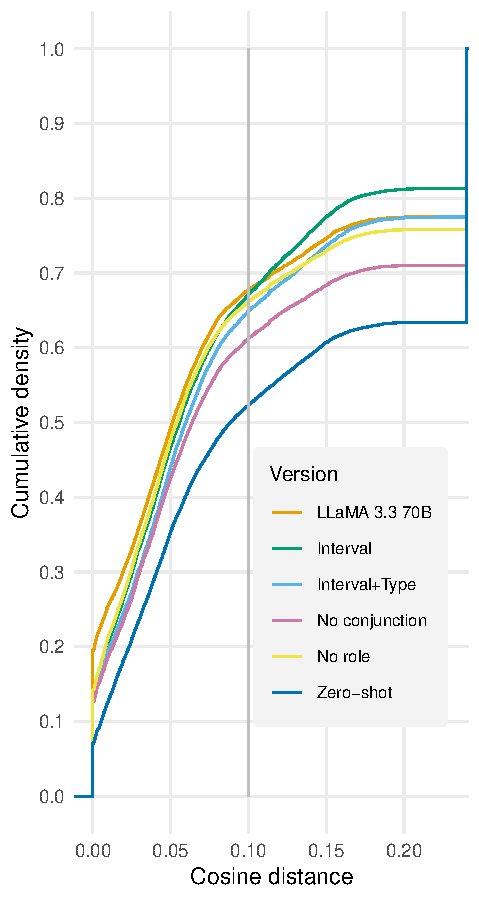
\includegraphics[page=1, width=\linewidth]{Plots_tables/prompt_ablation_updated_figure.pdf}
    \end{minipage}
    \hfill
    \begin{minipage}[t]{0.242\textwidth}
    \centering
    \includegraphics[page=2, width=\linewidth]{Plots_tables/prompt_ablation_updated_figure.pdf}
    \end{minipage}
    \hfill
    \begin{minipage}[t]{0.242\textwidth}
    \centering
    \includegraphics[page=3, width=\linewidth]{Plots_tables/prompt_ablation_updated_figure.pdf}
    \end{minipage}
    \hfill
    \begin{minipage}[t]{0.242\textwidth}
    \centering
    \includegraphics[page=4, width=\linewidth]{Plots_tables/prompt_ablation_updated_figure.pdf}
    \end{minipage}
    \caption{Comparison of \texttt{Llama 3.3 70B} prompt ablation and variant methods for extracting temporal clinical events from case reports. From left to right: (\textbf{A}) event match cumulative distribution function, (\textbf{B}) concordance box plots, (\textbf{C}) time discrepancy from manual annotation timestamps among matched events (overall), and (\textbf{D}) time discrepancy disaggregated by clinician annotator timestamp (time from presentation).}
    \label{fig:prompt_ablation}
    \vspace{-5mm}
\end{figure}



\paragraph{Semantic similarity:}
The cumulative density of cosine distances between matched events reveals that omitting key components of the prompt negatively impacts text alignment (Figure \ref{fig:prompt_ablation}, left). The Interval, \texttt{DSR1}, and Interval+Type prompts consistently show high-quality event matches, with over 80\% of events falling below a cosine distance of 0.1. In contrast, removing role framing (No role) or conjunction splitting (No conjunction) leads to modest degradation. The Zero-shot condition—lacking both examples and guiding instructions—performs markedly worse, with only ~60\% of events under the same similarity threshold.

\paragraph{Temporal concordance:} Concordance index (c-index) measures the agreement between predicted and annotated event ordering (Figure \ref{fig:prompt_ablation}, middle left). The Interval+Type variant achieves the highest median concordance, followed closely by Interval, \texttt{DSR1}, and No role. Removing conjunction expansion reduces ordering consistency slightly, while Zero-shot again yields the lowest performance with a wider spread and multiple outliers (c-index < 0.6), indicating inconsistent temporal sequencing.

\paragraph{Timestamp discrepancy:} Cumulative distributions of time discrepancies from manual annotations further support these findings (Figure \ref{fig:prompt_ablation}, middle right). Structured prompts—especially Interval, \texttt{DSR1}, and Interval+Type—demonstrate tighter timestamp alignment. Ablations involving role removal or conjunction omission produce broader error distributions, and Zero-shot extraction results in substantially larger timestamp mismatches.

When stratified by the time from presentation (e.g., within 1 hour, 1 day, 1 week), prompt differences are most pronounced for events occurring farther from the report anchor (Figure \ref{fig:prompt_ablation}, far right). For immediate events, all prompt versions perform comparably. However, at longer timescales (1 week to "ever"), Interval and Interval+Type maintain superior accuracy, while Zero-shot shows dramatic drops in performance. This suggests that structured prompts are particularly critical for accurate long-range temporal reasoning.

%%%%%%%%%%%%%%%%%%%%%%%%%%%%%%%%%%%%%
%%%%%%%%%%%%%%%%%%%%%%%%%%%%%%%%%%%%%

\subsection{Inter-LLM comparison of temporal annotations} \textcolor{red}{Move to Appendix?}
%\label{apd:example_annotations}

In this section, we showcase an excerpt from case report with PMC ID 10629858 \citep{abu2023rare}. To demonstrate the extraction task and analyze the performance of various LLM annotators, we compare manual annotations against outputs from several LLM variants: \texttt{DeepSeek-R1}, \texttt{DeepSeek-V3-0324}, \texttt{LLaMA 3.3 70B}, \texttt{OpenAI GPT5}, \texttt{OpenAI O1}, \texttt{OpenAI O3}, and \texttt{OpenAI O4-mini} (Figure \ref{fig:compare_llm_annotations}).

% \noindent\textcolor{red}{Multi-LLM examples go into Appendix \ref{fig:compare_LLM_annotations}}. 
% \textcolor{red}{Add a table with error types or few example errors (similar to Fig 3 in Jing's AMIA IS paper)}
%\newcolumntype{P}[1]{>{\raggedright\hangindent=1em\hangafter=1}p{#1}}
\begin{figure*}[t]
    Excerpt from \cite{abu2023rare}:
    \begin{quote}\footnotesize
    A 57-year-old man recently diagnosed with lepromatous leprosy was confirmed with skin biopsy and had been on treatment (rifampicin/clofazimine/dapsone) for 2 months before admission; he was presented to the hospital with complaints of abdominal distension, constipation, vomiting, and a 10-kg weight loss. On examination, the patient was vitally stable. He had evidence of peripheral lymphadenopathy with a distended abdomen and a positive shifting dullness. A computed tomography scan of his abdomen showed mural thickening of the terminal ileum with significantly enlarged mesenteric lymph nodes, mesenteric fat stranding, and intra-abdominal free fluid, suggesting abdominal granulomatous infection or neoplastic process.
    \dots 
    
    The patient was planned for consolidation by autologous bone marrow transplant. Unfortunately, with the recurrent bacteremia and sepsis that accompanied the patient’s course due to his immunocompromised state, he was re-admitted to the medical ICU for severe sepsis and multiorgan failure and passed away around 6 months after his initial diagnosis with NHL, despite maintaining a remission status.
    \end{quote}

    % DeepSeek-R1, DeepSeek-R1-UD-IQ1, DeepSeek-V3-
    % 0324, LLaMA 3.3 70B, OpenAI O1, OpenAI O3, and OpenAI O4-mini

    %%%%%%%%%%%%%%%%%%%%%%%%%%%%%%%%%%%%%%%%%%%%%%%%%%%%%%%%
    %%%%%%%% Manual and DeepSeek R1 %%%%%%%%%%%%%%%%%%%%%%%%%%%%%%
    %%%%%%%%%%%%%%%%%%%%%%%%%%%%%%%%%%%%%%%%%%%%%%%%%%%%%%%%

    \begin{minipage}[!htbp]{0.49\textwidth}
    \footnotesize
        \textbf{Manual annotation} \\ \\
        \footnotesize
        \begin{tabular}{P{0.75\textwidth}r}
            57-year-old&0 \\
            man&0 \\
            diagnosed with lepromatous leprosy&-1461 \\
            on treatment&-1461 \\
            rifampicin&-1461 \\
            clofazimine&-1461 \\
            dapsone&-1461 \\
            presented to the hospital&0 \\
            abdominal distension&0 \\
            constipation&0 \\
            vomiting&0 \\
            10-kg weight loss&0 \\
            vitally stable&0 \\
            peripheral lymphadenopathy&0 \\
            distended abdomen&0 \\
            positive shifting dullness&0 \\
            computed tomography scan of his abdomen&0 \\
            mural thickening of the terminal ileum&0 \\
            significantly enlarged mesenteric lymph nodes&0 \\
            mesenteric fat stranding&0 \\
            intra-abdominal free fluid&0 \\
            % Abdominal paracentesis&0 \\
            re-admitted to the medical ICU&4383 \\
            severe sepsis&4383 \\
            multiorgan failure&4383 \\
            passed away&4383
        \end{tabular}
    \end{minipage}
    \begin{minipage}[!htbp]{0.49\textwidth}
    \footnotesize
        \textbf{DeepSeek-R1 annotation} \\ \\
        \footnotesize
        \begin{tabular}{P{0.75\textwidth}r}
            57 years old & 0 \\
            male & 0 \\
            lepromatous leprosy & -1464 \\
            skin biopsy & -1464 \\
            rifampicin & -1464 \\
            clofazimine & -1464 \\
            dapsone & -1464 \\
            admitted to the hospital & 0 \\
            abdominal distension & 0 \\
            constipation & 0 \\
            vomiting & 0 \\
            10-kg weight loss & 0 \\
            vital stability & 0 \\
            peripheral lymphadenopathy & 0 \\
            distended abdomen & 0 \\
            positive shifting dullness & 0 \\
            computed tomography scan & 0 \\
            mural thickening of the terminal ileum & 0 \\
            enlarged mesenteric lymph nodes & 0 \\
            mesenteric fat stranding & 0 \\
            intra-abdominal free fluid & 0 \\
            abdominal paracentesis & 0 \\
            plan for autologous bone marrow transplant & 4320 \\
            recurrent bacteremia & 4320 \\
            sepsis & 4320 \\
            readmission to ICU & 4320 \\
            severe sepsis & 4320 \\
            multiorgan failure & 4320 \\
            death & 4320 \\
            & 
        \end{tabular}
    \end{minipage}

\end{figure*}

%%%%%%%%%%%%%%%%%%%%%%%%%%%%%%%%%%%%%%%%%%%%%%%%%%%%%%%%
%%%%%%%%  DeepSeek-V3 and Llama 3.3 70B %%%%%%
%%%%%%%%%%%%%%%%%%%%%%%%%%%%%%%%%%%%%%%%%%%%%%%%%%%%%%%%
\begin{figure*}[!htbp]
    \begin{minipage}[!htbp]{0.49\textwidth}
    \footnotesize
        \textbf{DeepSeek-V3-0324 annotation} \\ \\
        \footnotesize
        \begin{tabular}{P{0.75\textwidth}r}
            57 years old & 0 \\
            male & 0 \\
            lepromatous leprosy & -1464 \\
            skin biopsy & -1464 \\
            rifampicin & -1464 \\
            clofazimine & -1464 \\
            dapsone & -1464 \\
            admitted to the hospital & 0 \\
            abdominal distension & 0 \\
            constipation & 0 \\
            vomiting & 0 \\
            weight loss & 0 \\
            peripheral lymphadenopathy & 0 \\
            distended abdomen & 0 \\
            positive shifting dullness & 0 \\
            computed tomography scan & 0 \\
            mural thickening of the terminal ileum & 0 \\
            enlarged mesenteric lymph nodes & 0 \\
            mesenteric fat stranding & 0 \\
            intra-abdominal free fluid & 0 \\
            abdominal granulomatous infection & 0 \\
            neoplastic process & 0 \\
            abdominal paracentesis & 0 \\
            autologous bone marrow transplant planned & 672 \\
            recurrent bacteremia & 672 \\
            sepsis & 672 \\
            re-admitted to the medical ICU & 4032 \\
            severe sepsis & 4032 \\
            multiorgan failure & 4032 \\
            passed away & 4032 \\
            complete metabolic remission & 4032 \\
        \end{tabular}
    \end{minipage}
    \begin{minipage}[!htbp]{0.49\textwidth}
    \footnotesize
        \textbf{LLaMA 3.3 70B annotation} \\ \\
        \footnotesize
        \begin{tabular}{P{0.75\textwidth}r}
            57 years old & 0 \\
            male & 0 \\
            lepromatous leprosy & -144 \\
            skin biopsy & -144 \\
            rifampicin & -144 \\
            clofazimine & -144 \\
            dapsone & -144 \\
            abdominal distension & 0 \\
            constipation & 0 \\
            vomiting & 0 \\
            weight loss & 0 \\
            peripheral lymphadenopathy & 0 \\
            distended abdomen & 0 \\
            positive shifting dullness & 0 \\
            mural thickening of the terminal ileum & 0 \\
            enlarged mesenteric lymph nodes & 0 \\
            mesenteric fat stranding & 0 \\
            intra-abdominal free fluid & 0 \\
            abdominal granulomatous infection & 0 \\
            neoplastic process & 0 \\
            autologous bone marrow transplant & 1344 \\
            recurrent bacteremia & 1344 \\
            sepsis & 1344 \\
            multiorgan failure & 1344 \\
            passed away & 1440 \\
            & 
        \end{tabular}
    \end{minipage}
\end{figure*}
%%%%%%%%%%%%%%%%%%%%%%%%%%%%%%%%%%%%%%%%%%%%%%%%%%%%%%%%
%%%%%%%% GPT5 and O1 %%%%%%%%%%%%%%%%%%%%%%%%%%%%%%
%%%%%%%%%%%%%%%%%%%%%%%%%%%%%%%%%%%%%%%%%%%%%%%%%%%%%%%%
\begin{figure*}[!htbp]
    \begin{minipage}[!htbp]{0.49\textwidth}
    \footnotesize
        \textbf{GPT5 annotation} \\ \\
        \footnotesize
        \begin{tabular}{P{0.75\textwidth}r}
            57-year-old man & 0 \\
            male & 0 \\
            recently diagnosed with lepromatous leprosy & -1440 \\
            skin biopsy confirmed lepromatous leprosy & -1440 \\
            rifampicin started & -1440 \\
            clofazimine started & -1440 \\
            dapsone started & -1440 \\
            presented to the hospital with complaints of abdominal distension & 0 \\
            constipation & 0 \\
            vomiting & 0 \\
            10-kg weight loss & 0 \\
            peripheral lymphadenopathy & 0 \\
            distended abdomen & 0 \\
            positive shifting dullness & 0 \\
            computed tomography scan of his abdomen & 6\\
            mural thickening of the terminal ileum & 6 \\
            significantly enlarged mesenteric lymph nodes & 6 \\
            mesenteric fat stranding & 6 \\
            intra-abdominal free fluid & 6 \\
            abdominal granulomatous infection or neoplastic process suggested & 6 \\
            abdominal paracentesis was done & 6 \\
            recurrent bacteremia & 1200 \\
            % neoplastic process & 0 \\
            planned for consolidation by autologous bone marrow transplant & 2400 \\
            remission status maintained & 4200 \\
            re-admitted to the medical ICU for severe sepsis and multiorgan failure & 4296 \\
            passed away & 4320 \\
        \end{tabular}
    \end{minipage}
    \begin{minipage}[!htbp]{0.49\textwidth}
    \footnotesize
        \textbf{OpenAI O1 annotation} \\ \\
        \footnotesize
        \begin{tabular}{P{0.75\textwidth}r}
            % 57 years old & -1440 \\
            % male & -1440 \\
            diagnosed with lepromatous leprosy & -1344 \\  
            confirmed with skin biopsy & -1344 \\  
            treatment with rifampicin/clofazimine/dapsone & -1344 \\  
            admitted to the hospital & 0 \\ 
            vitally stable & 0 \\
            abdominal distension & 0 \\  
            constipation & 0 \\  
            vomiting & 0 \\ 
            10-kg weight loss & 0 \\   
            peripheral lymphadenopathy & 0 \\  
            distended abdomen & 0 \\  
            positive shifting dullness & 0 \\  
            computed tomography scan & 0 \\  
            mural thickening of the terminal ileum & 0 \\  
            significantly enlarged mesenteric lymph nodes & 0 \\  
            mesenteric fat stranding & 0 \\  
            intra-abdominal free fluid & 0 \\  
            suggesting abdominal granulomatous infection or neoplastic process & 0 \\  
            abdominal paracentesis & 0 \\ 
            % Planned for consolidation by autologous bone marrow transplant & 2136  \\
            % Responded well to chemotherapy & 2280   \\
            % Attained complete metabolic remission by positron emission tomography/computed tomography & 2280   \\
            planned for consolidation by autologous bone marrow transplant & 2500 \\  
            re-admitted to the medical ICU  & 3000 \\  
            severe sepsis &	3000 \\
            multiorgan failure & 3000 \\
            passed away & 4320 \\
            & 
        \end{tabular}
    \end{minipage}
\end{figure*} 

%%%%%%%%%%%%%%%%%%%%%%%%%%%%%%%%%%%%%%%%%%%%%%%%%%%%%%%%
%%%%%%%% O3 and O4-mini %%%%%%%%%%%%%%%%%%%%%%%%%%%%%%
%%%%%%%%%%%%%%%%%%%%%%%%%%%%%%%%%%%%%%%%%%%%%%%%%%%%%%%%
\begin{figure*}[!htbp]
    \begin{minipage}[!htbp]{0.49\textwidth}
    \footnotesize
        \textbf{OpenAI O3 annotation} \\ \\
        \footnotesize
        \begin{tabular}{P{0.75\textwidth}r}
            lepromatous leprosy diagnosis & -1440 \\
            skin biopsy confirmed lepromatous leprosy & -1440 \\
            rifampicin treatment started & -1440 \\
            clofazimine treatment started & -1440 \\
            dapsone treatment started & -1440 \\
            presented to hospital & 0 \\
            abdominal distension & 0 \\
            constipation & 0 \\
            vomiting & 0 \\
            10-kg weight loss & 0 \\
            vitally stable & 0 \\
            peripheral lymphadenopathy & 0 \\
            distended abdomen & 0 \\
            positive shifting dullness & 0 \\
            computed tomography abdomen & 0 \\
            mural thickening of terminal ileum & 0 \\
            enlarged mesenteric lymph nodes & 0 \\
            mesenteric fat stranding & 0 \\
            intra-abdominal free fluid & 0 \\
            abdominal granulomatous infection suggested & 0 \\
            neoplastic process suggested & 0 \\
            abdominal paracentesis & 0 \\
            planned autologous bone marrow transplant & 2150 \\
            % assessment after four cycles & 2208 \\
            % complete metabolic remission on PET/CT & 2208 \\
            re‑admission to medical ICU & 4320 \\
            severe sepsis & 4320 \\
            multiorgan failure & 4320 \\
            death & 4320 \\
            remission status maintained & 4320
        \end{tabular}
    \end{minipage}
    \begin{minipage}[!htbp]{0.49\textwidth}
    \footnotesize
        \textbf{OpenAI O4-mini annotation} \\ \\
        \footnotesize
        \begin{tabular}{P{0.75\textwidth}r}
            lepromatous leprosy confirmed with skin biopsy & -1440 \\  
            rifampicin treatment started & -1440 \\  
            clofazimine treatment started & -1440 \\  
            dapsone treatment started & -1440 \\  
            57 years old & 0 \\  
            male & 0 \\ 
            presented to the hospital & 0 \\  
            complaint of abdominal distension & 0 \\  
            complaint of constipation & 0 \\  
            complaint of vomiting & 0 \\  
            10-kg weight loss & 0 \\  
            vitals stable & 0 \\  
            peripheral lymphadenopathy & 0 \\  
            distended abdomen & 0 \\  
            positive shifting dullness & 0 \\  
            mural thickening of the terminal ileum & 0 \\  
            significantly enlarged mesenteric lymph nodes & 0 \\  
            mesenteric fat stranding & 0 \\  
            intra-abdominal free fluid & 0 \\  
            abdominal paracentesis performed & 2 \\ 
            plan autologous bone marrow transplant & 1900 \\  
            %assessment after four cycles of EPOCH & 2256 \\  
            % response to chemotherapy achieved & 2256 \\  
            % complete metabolic remission attained by PET/CT &2256 \\  
            re-admission to medical ICU for severe sepsis and multiorgan failure & 4260 \\
            death & 4320 \\
            & 
        \end{tabular}
    \end{minipage}
    \caption{TTS comparison across multiple LLMs}
    \label{fig:compare_LLM_annotations}
\end{figure*}




\begin{figure}[!htbp]  % float page; will try to use its own page
  \centering
   %%%%%%%%%%%%%%%%%%%%%%%%%%%%%% 
    \begin{tcolorbox}[colback=white,colframe=black!30,boxrule=0.6pt,left=2mm,right=2mm,top=2mm,bottom=2mm,width=\linewidth]
    \footnotesize \textbf{Excerpt from \cite{abu2023rare}:}
    \begin{quote}\footnotesize
    A 57-year-old man recently diagnosed with lepromatous leprosy was confirmed with skin biopsy and had been on treatment (rifampicin/clofazimine/dapsone) for 2 months before admission; he was presented to the hospital with complaints of abdominal distension, constipation, vomiting, and a 10-kg weight loss. On examination, the patient was vitally stable. He had evidence of peripheral lymphadenopathy with a distended abdomen and a positive shifting dullness. A computed tomography scan of his abdomen showed mural thickening of the terminal ileum with significantly enlarged mesenteric lymph nodes, mesenteric fat stranding, and intra-abdominal free fluid, suggesting abdominal granulomatous infection or neoplastic process.
    \dots 
    
    The patient was planned for consolidation by autologous bone marrow transplant. Unfortunately, with the recurrent bacteremia and sepsis that accompanied the patient’s course due to his immunocompromised state, he was re-admitted to the medical ICU for severe sepsis and multiorgan failure and passed away around 6 months after his initial diagnosis with NHL, despite maintaining a remission status.
    \end{quote}
    \end{tcolorbox}
    %\vspace{2pt}
    %%%%%%%%%%%%%%%%%%%%%%%%%%%%%% 
  % Row 1
  \begin{subfigure}[!]{0.45\linewidth}\centering
    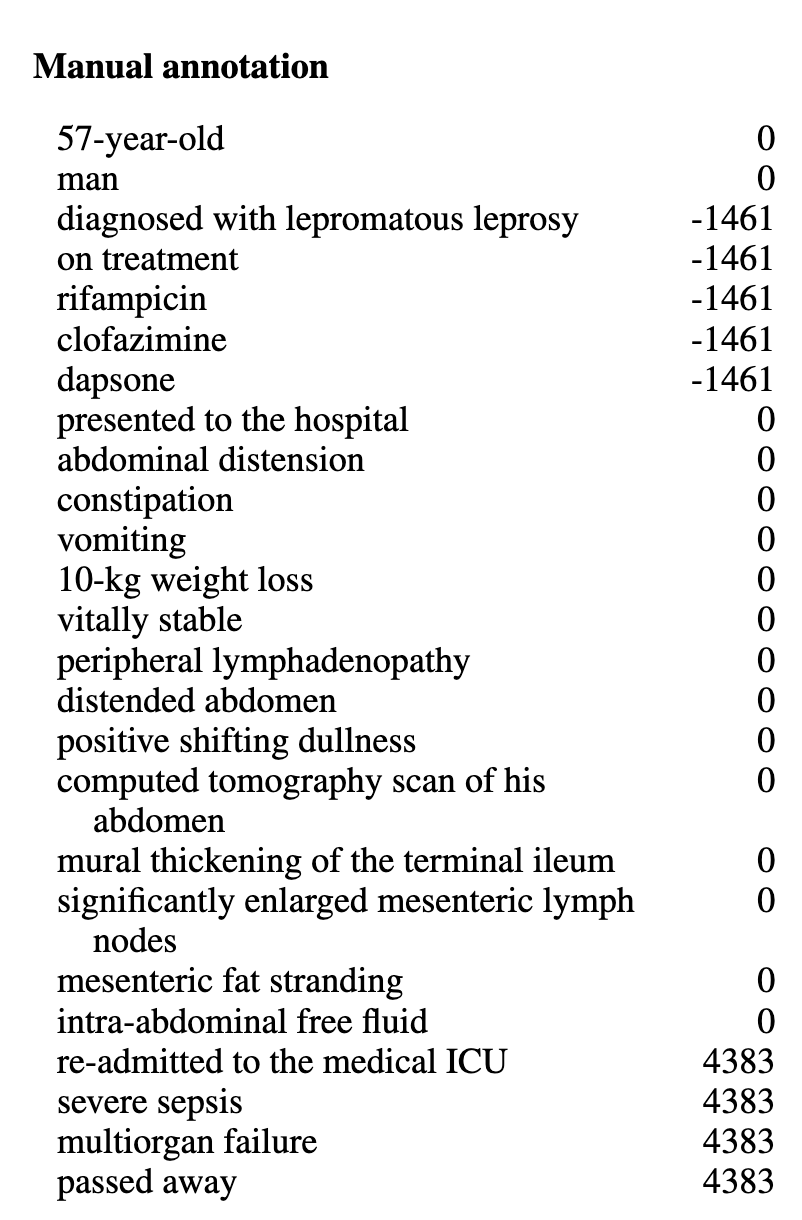
\includegraphics[width=0.9\linewidth]{Scientific_data/Supplementary/example_TTS_for_paper/manual.png}
    %\caption{...}\label{fig:a}
  \end{subfigure}\hfill
  \begin{subfigure}[!htbp]{0.45\linewidth}\centering
    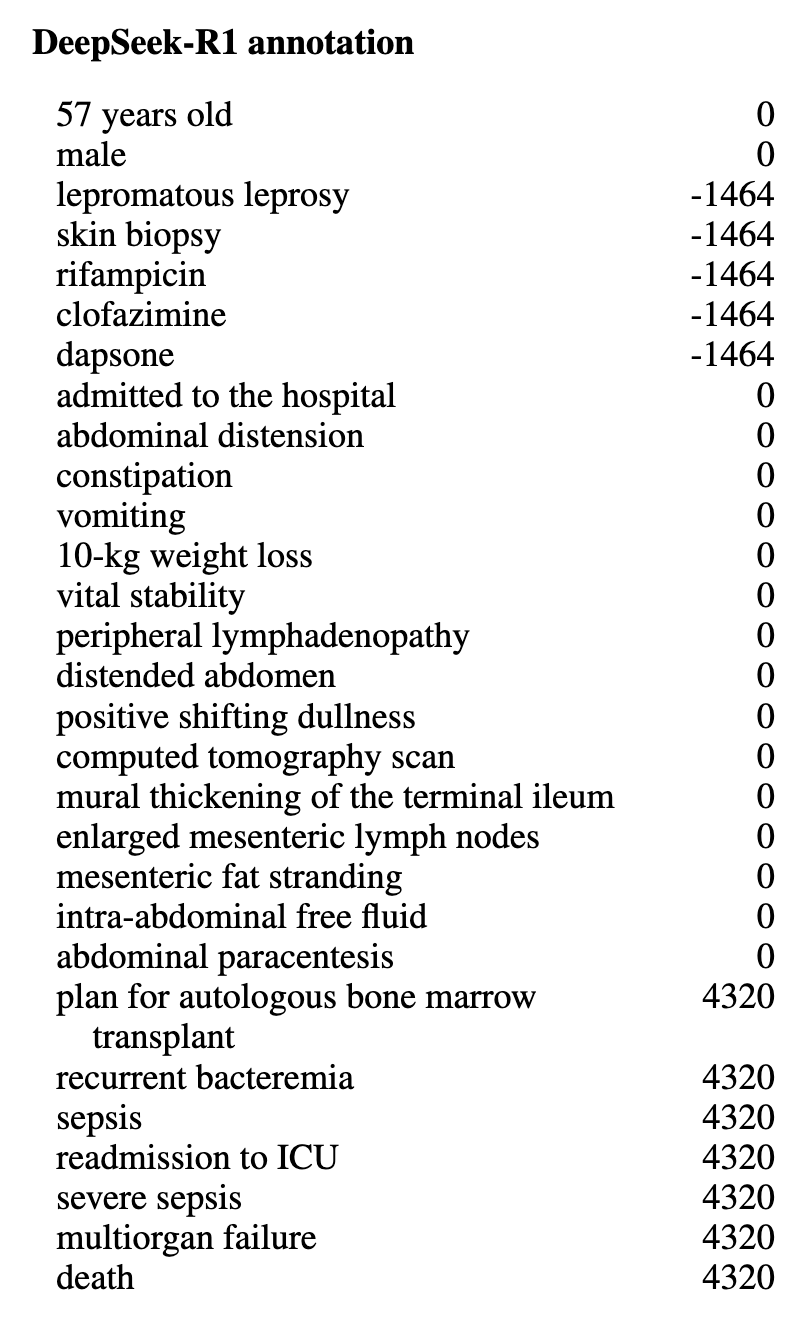
\includegraphics[width=0.9\linewidth]{Scientific_data/Supplementary/example_TTS_for_paper/DeepSeekR1.png}
    %\caption{...}\label{fig:b}
  \end{subfigure}

  %\vspace{6pt}

  % Row 2
  \begin{subfigure}[!htbp]{0.45\linewidth}\centering
    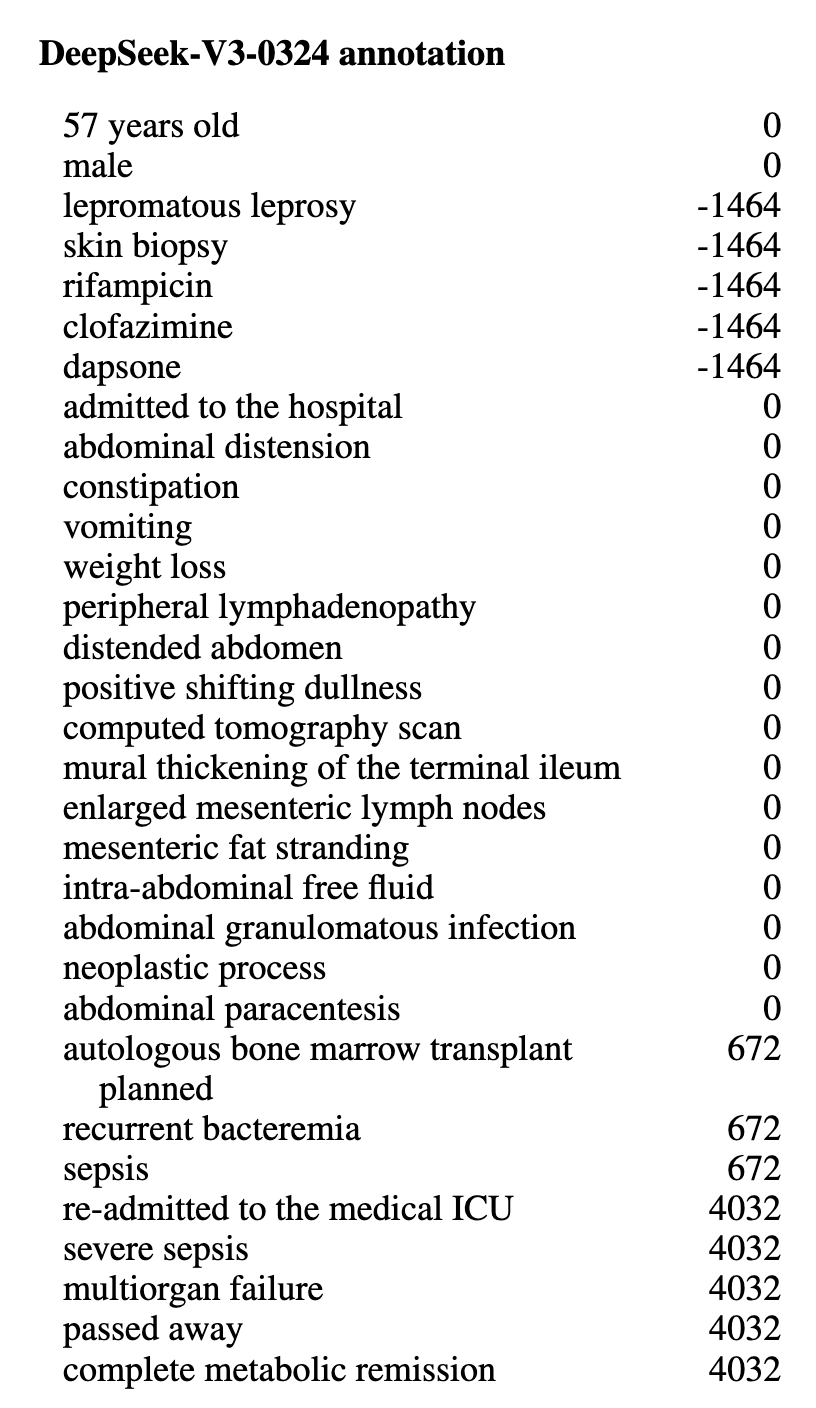
\includegraphics[width=0.9\linewidth]{Scientific_data/Supplementary/example_TTS_for_paper/DeepSeekV3.png}
    %\caption{...}\label{fig:c}
  \end{subfigure}\hfill
  \begin{subfigure}[!htbp]{0.45\linewidth}\centering
    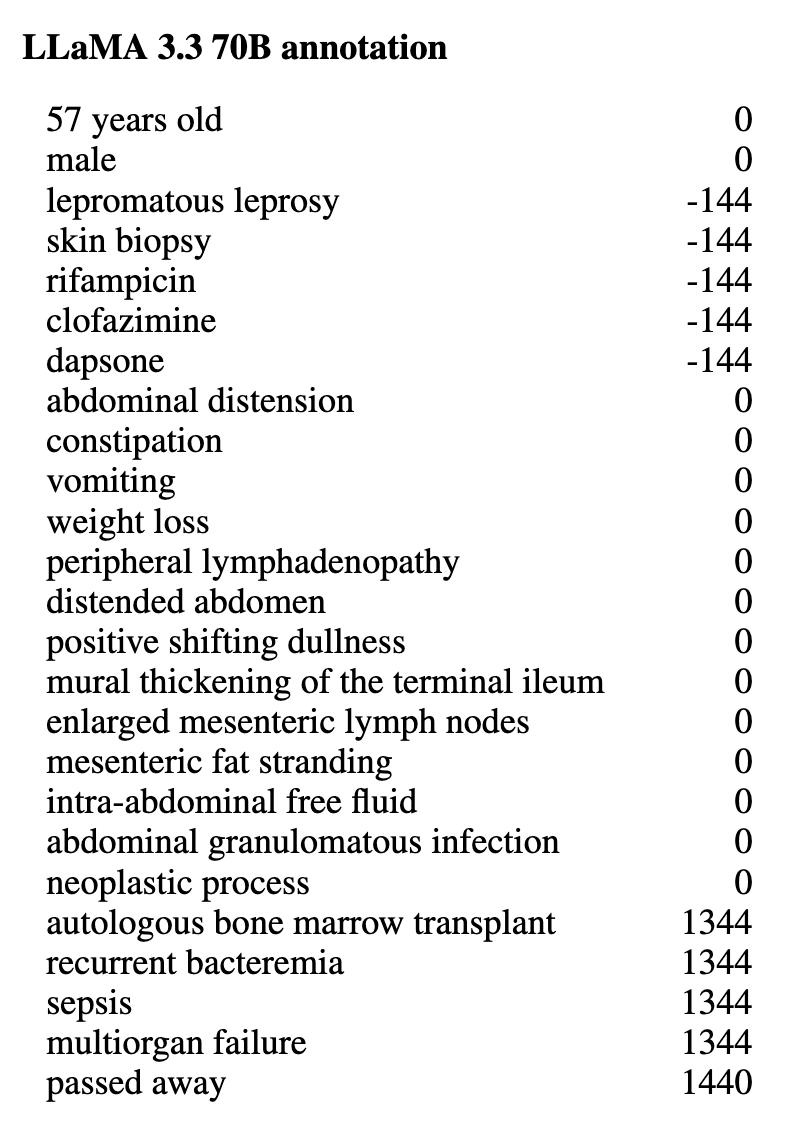
\includegraphics[width=0.9\linewidth]{Scientific_data/Supplementary/example_TTS_for_paper/L3370B.png}
    %\caption{...}\label{fig:d}
  \end{subfigure}
  %\caption{Overall caption for panels (a)–(d).}\label{fig:eight}
\end{figure}

%%%%%%%%%%%%%%%%%%%%%%%%%%%%%%%%%%%%%

\begin{figure}[!htbp]
  \centering
  % Row 1
  \begin{subfigure}[!htbp]{0.45\linewidth}\centering
    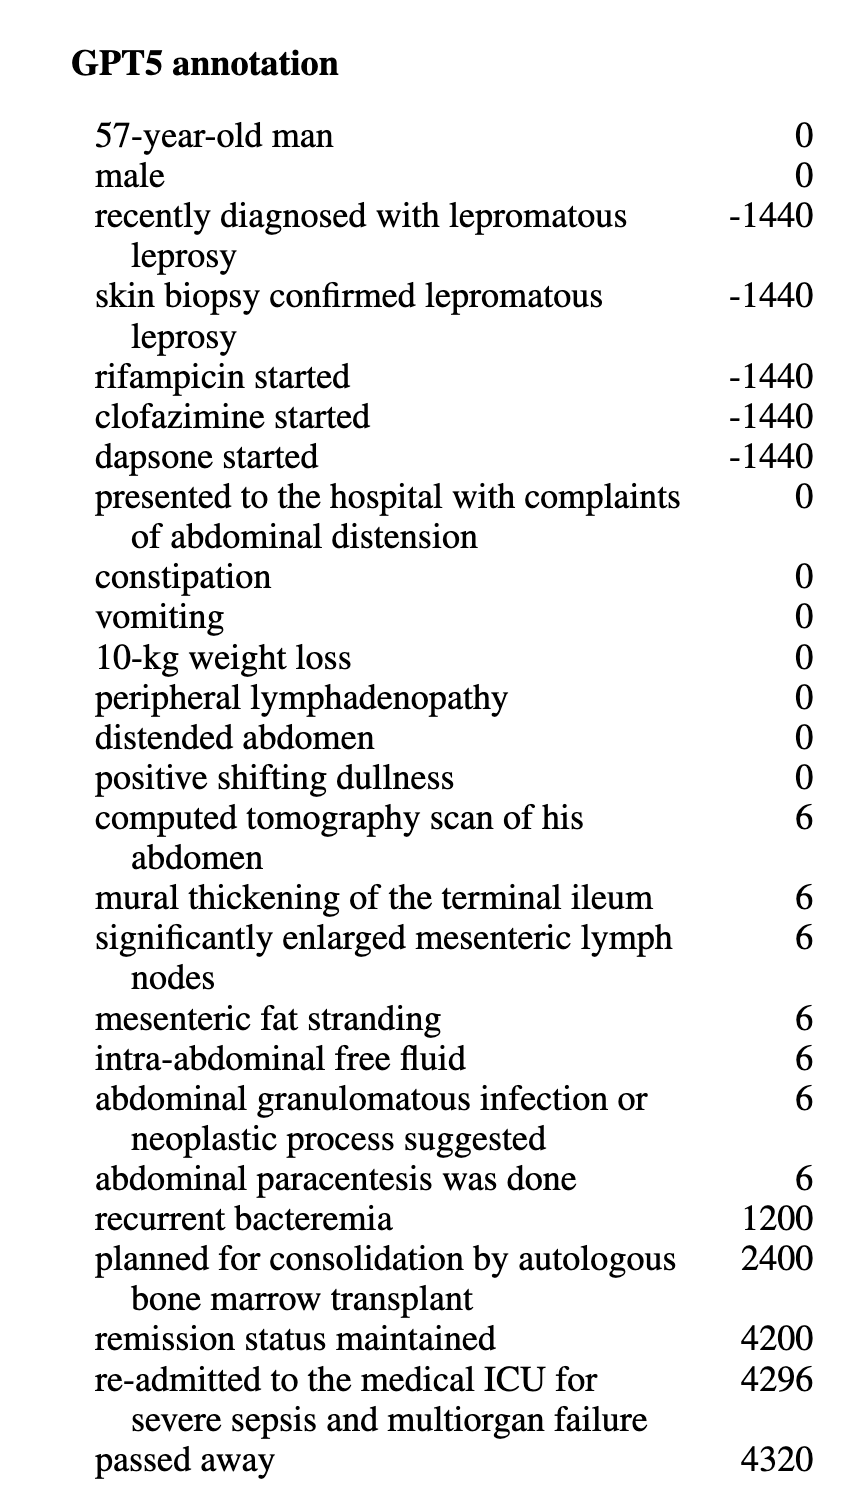
\includegraphics[width=0.9\linewidth]{Scientific_data/Supplementary/example_TTS_for_paper/GPT5.png}
    %\caption{...}\label{fig:e}
  \end{subfigure}\hfill
  \begin{subfigure}[!htbp]{0.45\linewidth}\centering
    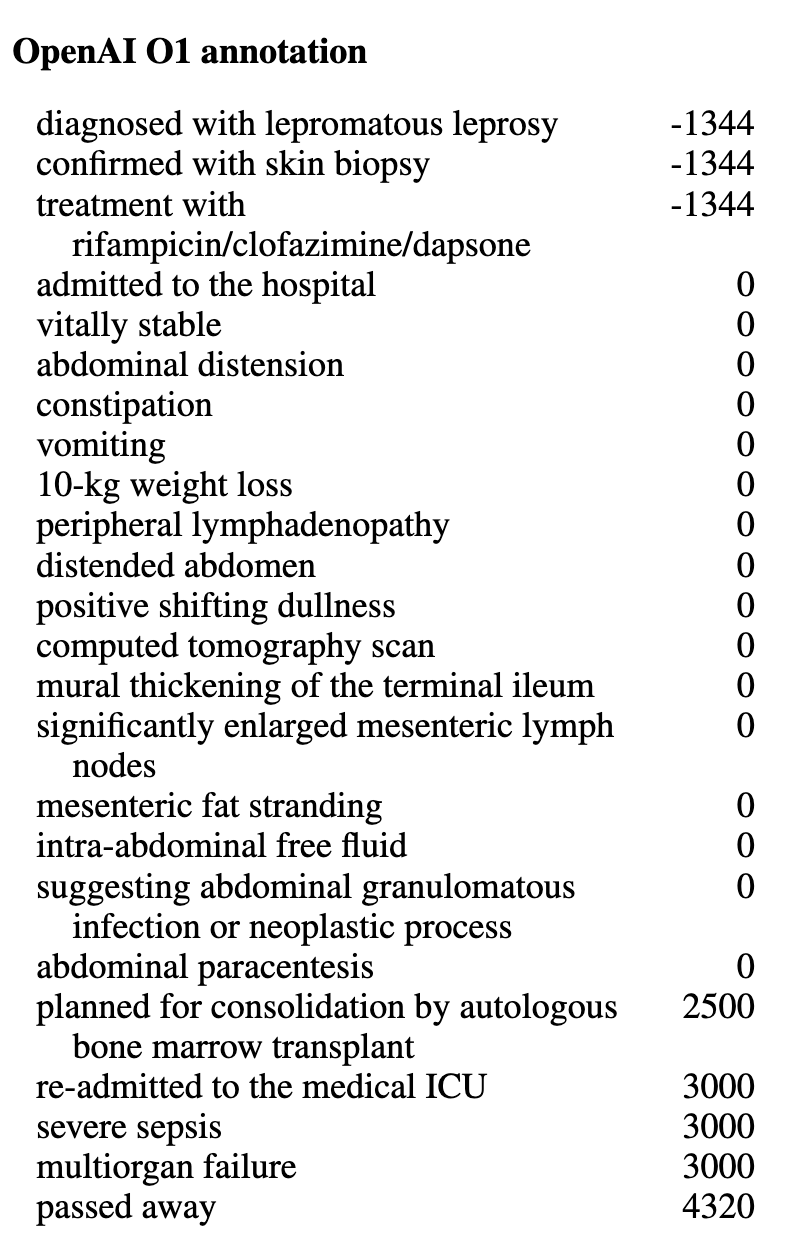
\includegraphics[width=0.9\linewidth]{Scientific_data/Supplementary/example_TTS_for_paper/O1.png}
    %\caption{...}\label{fig:f}
  \end{subfigure}

  \vspace{2pt}

  % Row 2
  \begin{subfigure}[!htbp]{0.45\linewidth}\centering
    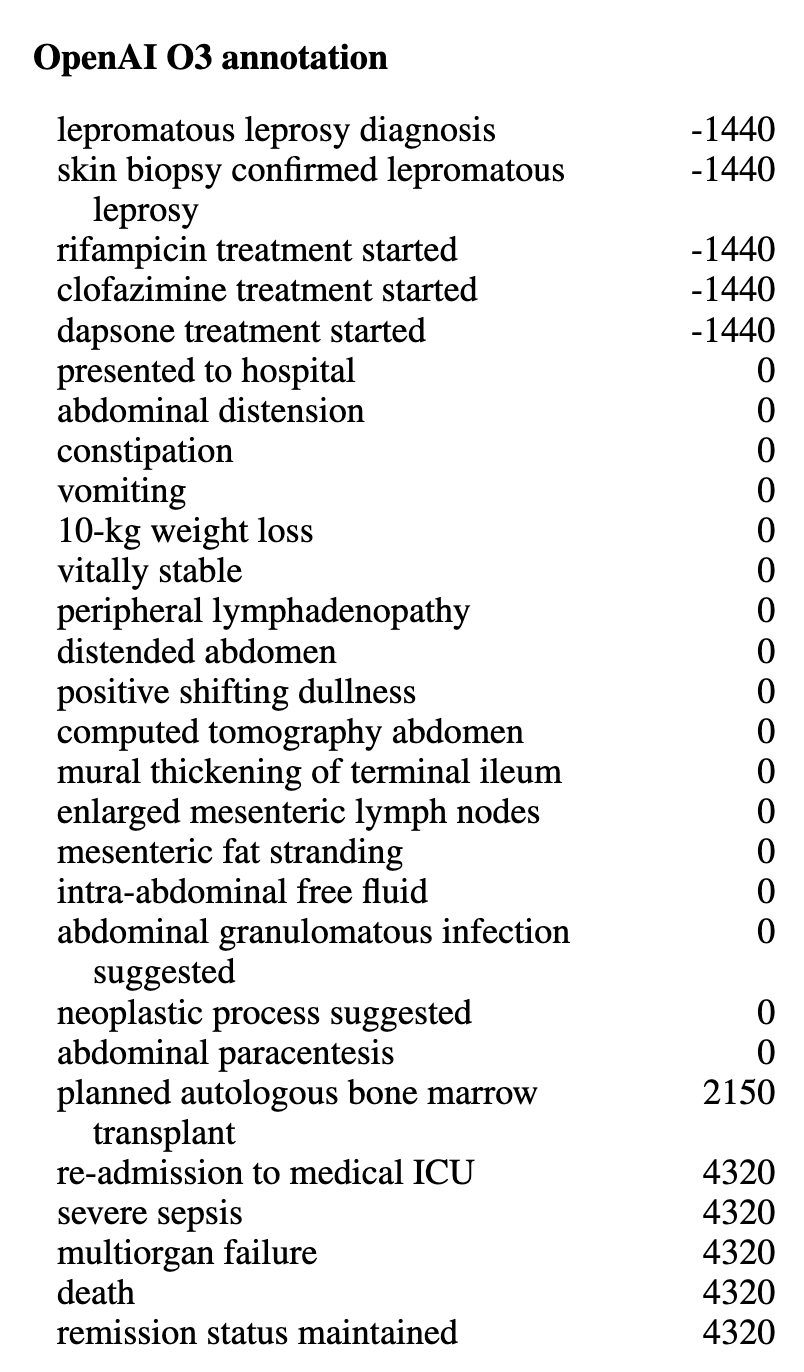
\includegraphics[width=0.9\linewidth]{Scientific_data/Supplementary/example_TTS_for_paper/O3.png}
    %\caption{...}\label{fig:g}
  \end{subfigure}\hfill
  \begin{subfigure}[!htbp]{0.45\linewidth}\centering
    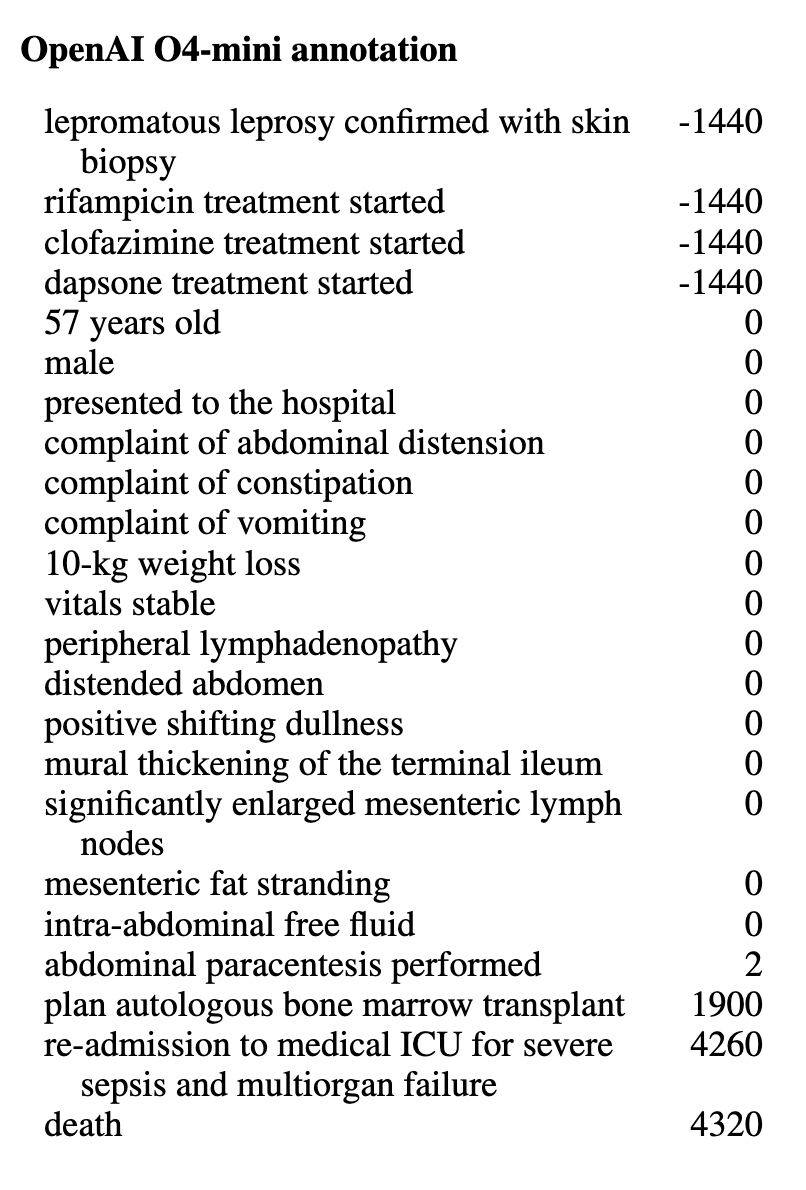
\includegraphics[width=0.9\linewidth]{Scientific_data/Supplementary/example_TTS_for_paper/O4mini.png}
    %\caption{...}\label{fig:h}
  \end{subfigure}

\caption{Comparison of temporal annotations generated by several LLMs for a representative case report (PMC10629858). The figure contrasts manual annotations with model-generated event–time
sequences, highlighting differences in event granularity, phrasing, duplicate event generation, and temporal normalization (e.g., variation in converting narrative expressions such as ``two
months before admission’’ into hour offsets). Long-range timestamp assignments (e.g., for transplant planning, ICU readmission, and death) show the greatest variability across models, whereas the overall ordering of major clinical events is largely preserved. This example illustrates characteristic
differences in how LLMs interpret, segment, and temporally anchor clinical narratives.}
  \label{fig:compare_llm_annotations}
  \vspace{-3mm}
\end{figure}


%%%%%%%%%%%%%%%%%%%%%%%%%%%%%%%%%%%%%%%%%
%%%%%%%%%%%%%%%%%%%%%%%%%%%%%%%%%%%%%%%%%

% \begin{figure*}[t]
% \centering

% % ---------------------------------------------------
% % Top: Excerpt box
% % ---------------------------------------------------
% \begin{tcolorbox}[
%   colback=white,
%   colframe=black!30,
%   boxrule=0.6pt,
%   left=2mm,right=2mm,top=2mm,bottom=2mm,
%   width=\linewidth
% ]
% \footnotesize \textbf{Excerpt from \cite{abu2023rare}:}
% \begin{quote}\footnotesize
% A 57-year-old man recently diagnosed with lepromatous leprosy was confirmed with skin biopsy 
% and had been on treatment (rifampicin/clofazimine/dapsone) for 2 months before admission; he 
% presented to the hospital with complaints of abdominal distension, constipation, vomiting, and 
% a 10-kg weight loss. On examination, the patient was vitally stable. He had evidence of peripheral 
% lymphadenopathy with a distended abdomen and a positive shifting dullness. A computed tomography 
% scan of his abdomen showed mural thickening of the terminal ileum with significantly enlarged 
% mesenteric lymph nodes, mesenteric fat stranding, and intra-abdominal free fluid, suggesting 
% abdominal granulomatous infection or neoplastic process. \dots

% The patient was planned for consolidation by autologous bone marrow transplant. Unfortunately, 
% with recurrent bacteremia and sepsis due to his immunocompromised state, he was re-admitted 
% to the medical ICU for severe sepsis and multiorgan failure and passed away around 6 months 
% after his initial diagnosis with NHL.
% \end{quote}
% \end{tcolorbox}

% \vspace{6pt}

% % ---------------------------------------------------
% % Grid of 8 subfigures (4 rows × 2 columns)
% % ---------------------------------------------------

% % Row 1
% \begin{subfigure}[t]{0.45\textwidth}
% \centering
% 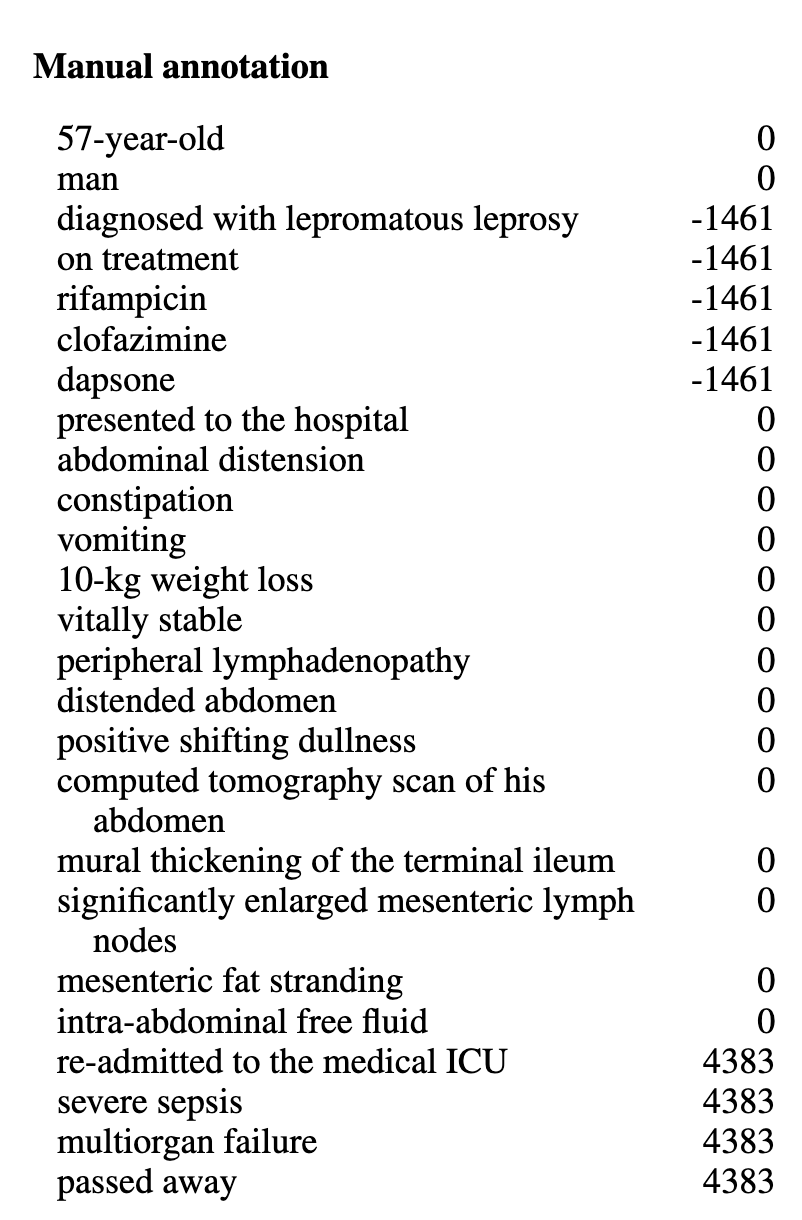
\includegraphics[width=0.95\linewidth]{Scientific_data/Supplementary/example_TTS_for_paper/manual.png}
% \caption*{Manual annotation}
% \end{subfigure}
% \hfill
% \begin{subfigure}[t]{0.45\textwidth}
% \centering
% 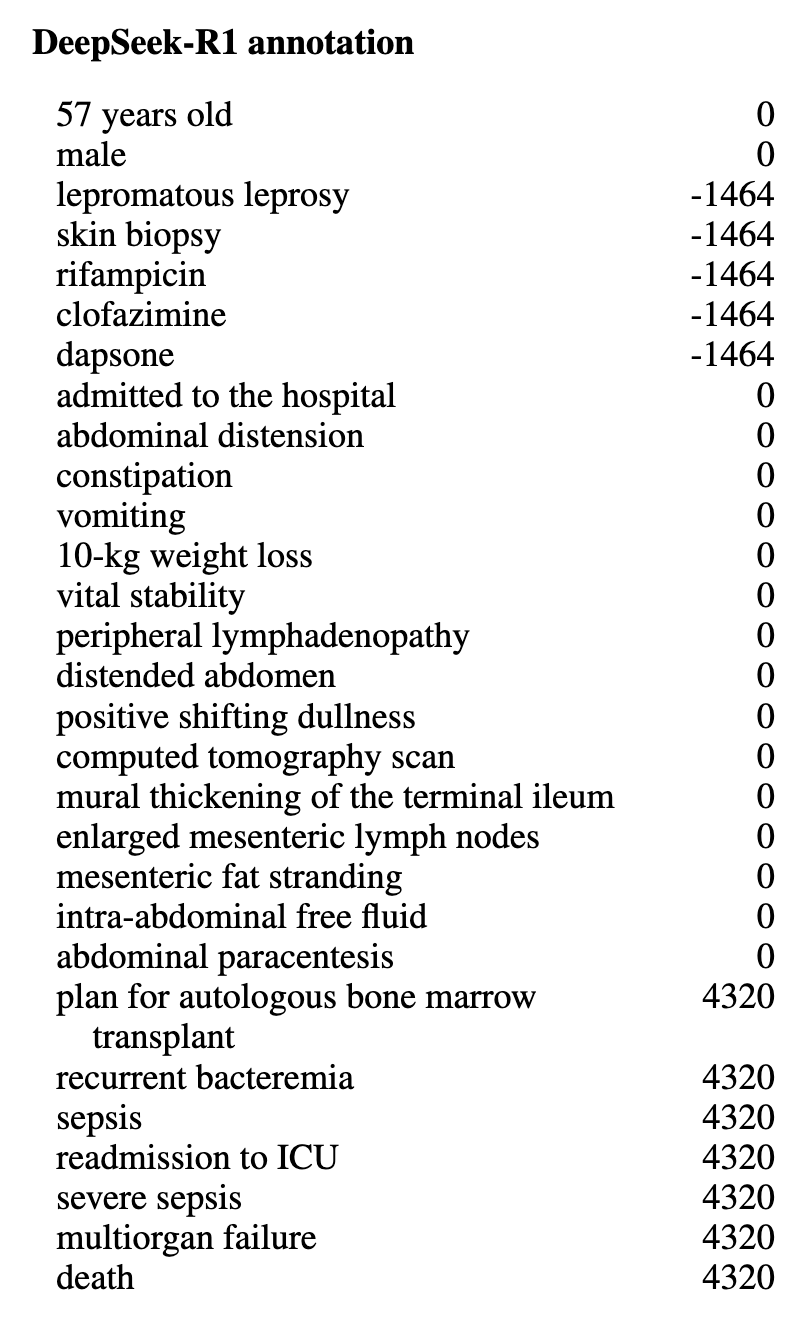
\includegraphics[width=0.95\linewidth]{Scientific_data/Supplementary/example_TTS_for_paper/DeepSeekR1.png}
% \caption*{\texttt{DeepSeek-R1}}
% \end{subfigure}

% \vspace{4pt}

% % Row 2
% \begin{subfigure}[t]{0.45\textwidth}
% \centering
% 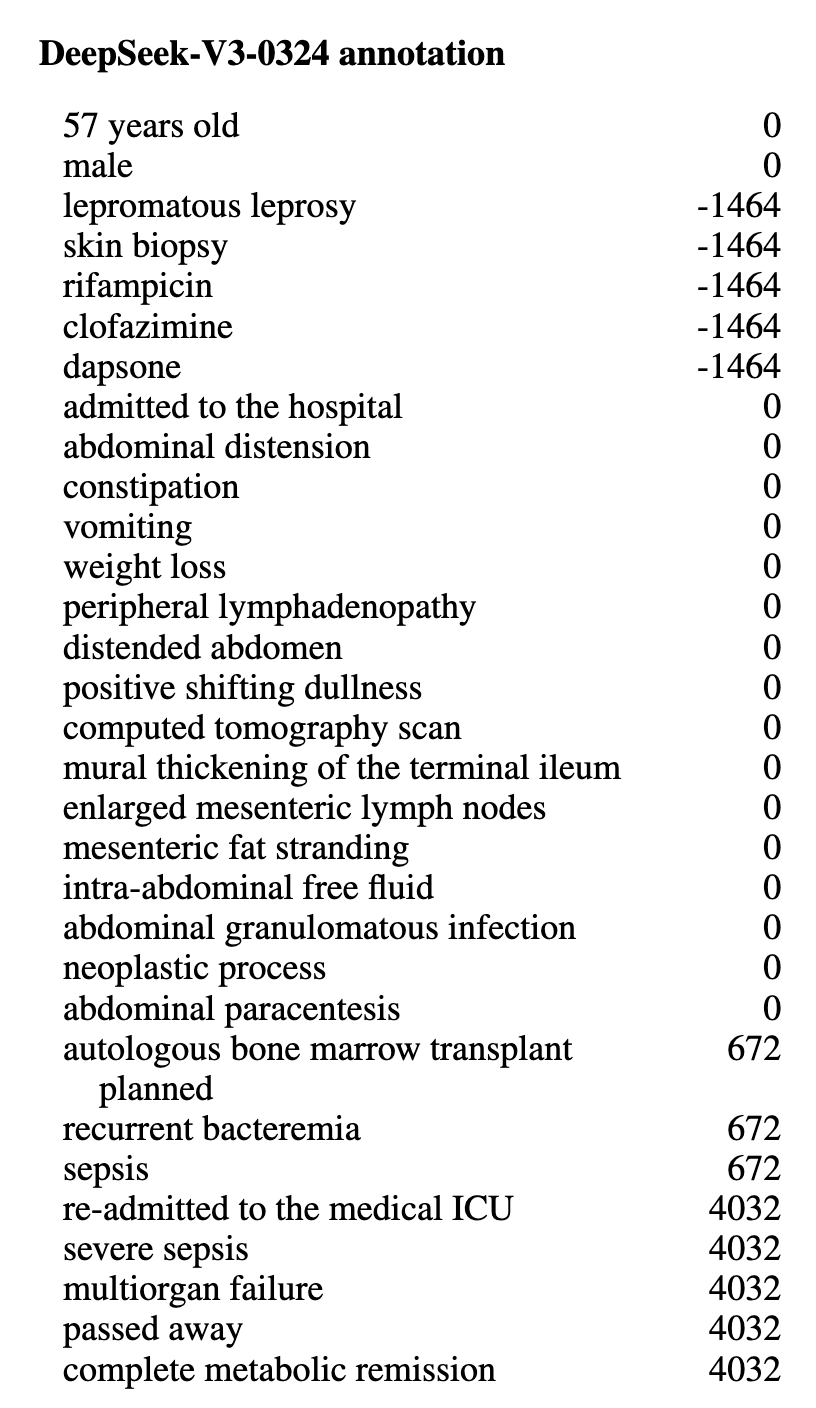
\includegraphics[width=0.95\linewidth]{Scientific_data/Supplementary/example_TTS_for_paper/DeepSeekV3.png}
% \caption*{\texttt{DeepSeek-V3-0324}}
% \end{subfigure}
% \hfill
% \begin{subfigure}[t]{0.45\textwidth}
% \centering
% 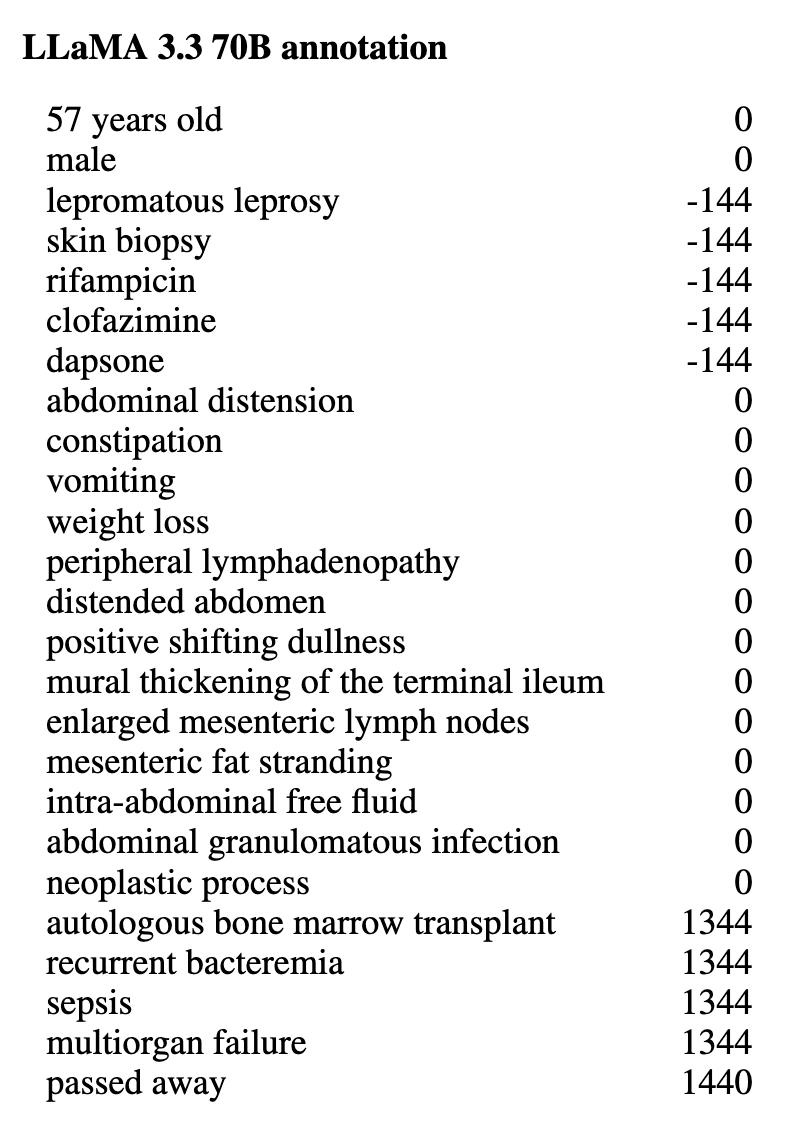
\includegraphics[width=0.95\linewidth]{Scientific_data/Supplementary/example_TTS_for_paper/L3370B.png}
% \caption*{\texttt{LLaMA~3.3~70B}}
% \end{subfigure}

% \vspace{4pt}

% % Row 3
% \begin{subfigure}[t]{0.45\textwidth}
% \centering
% 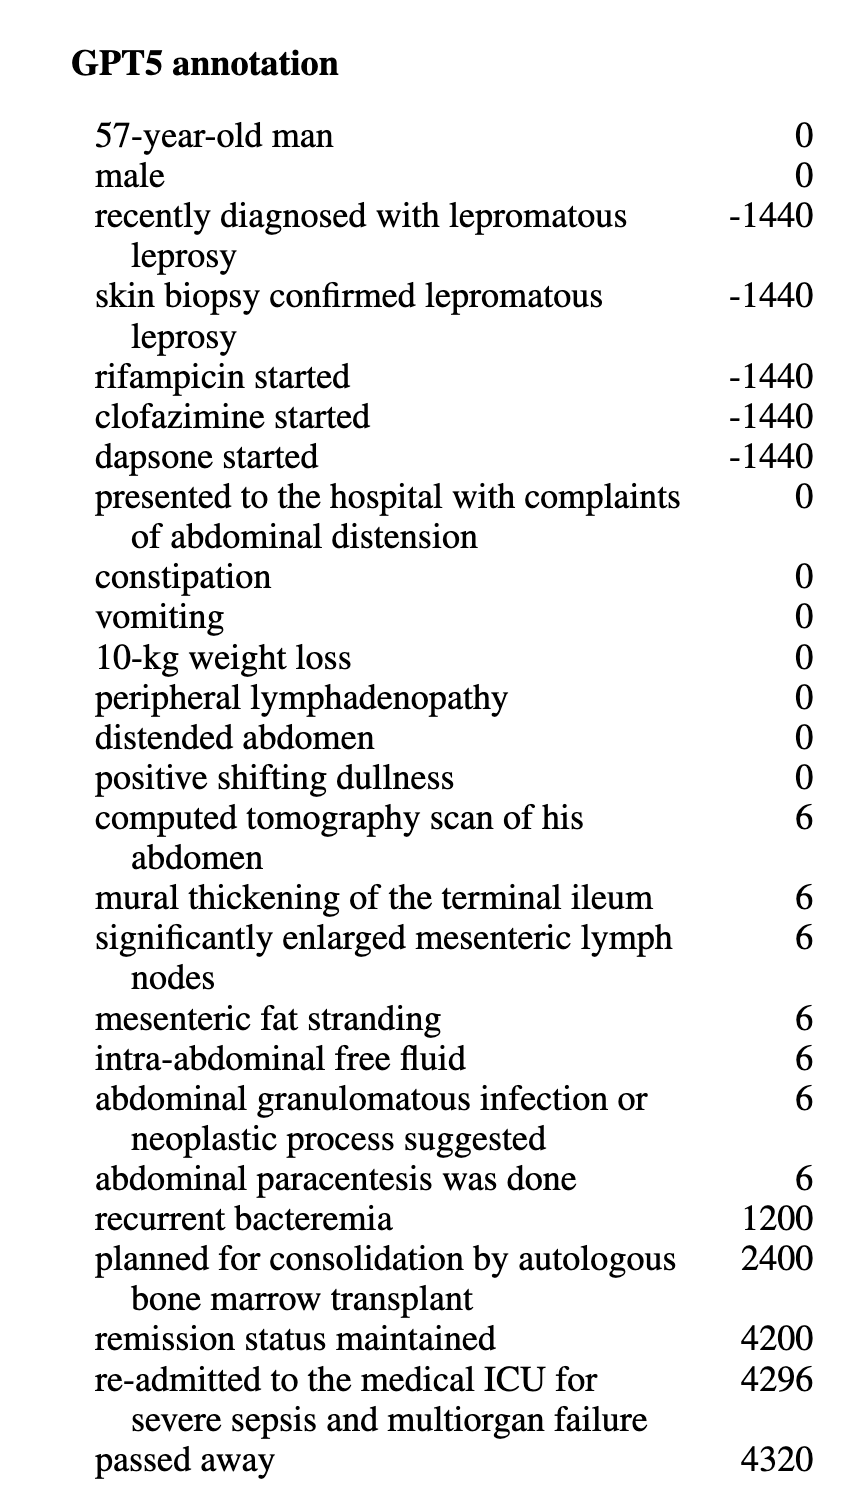
\includegraphics[width=0.95\linewidth]{Scientific_data/Supplementary/example_TTS_for_paper/GPT5.png}
% \caption*{\texttt{GPT5}}
% \end{subfigure}
% \hfill
% \begin{subfigure}[t]{0.45\textwidth}
% \centering
% 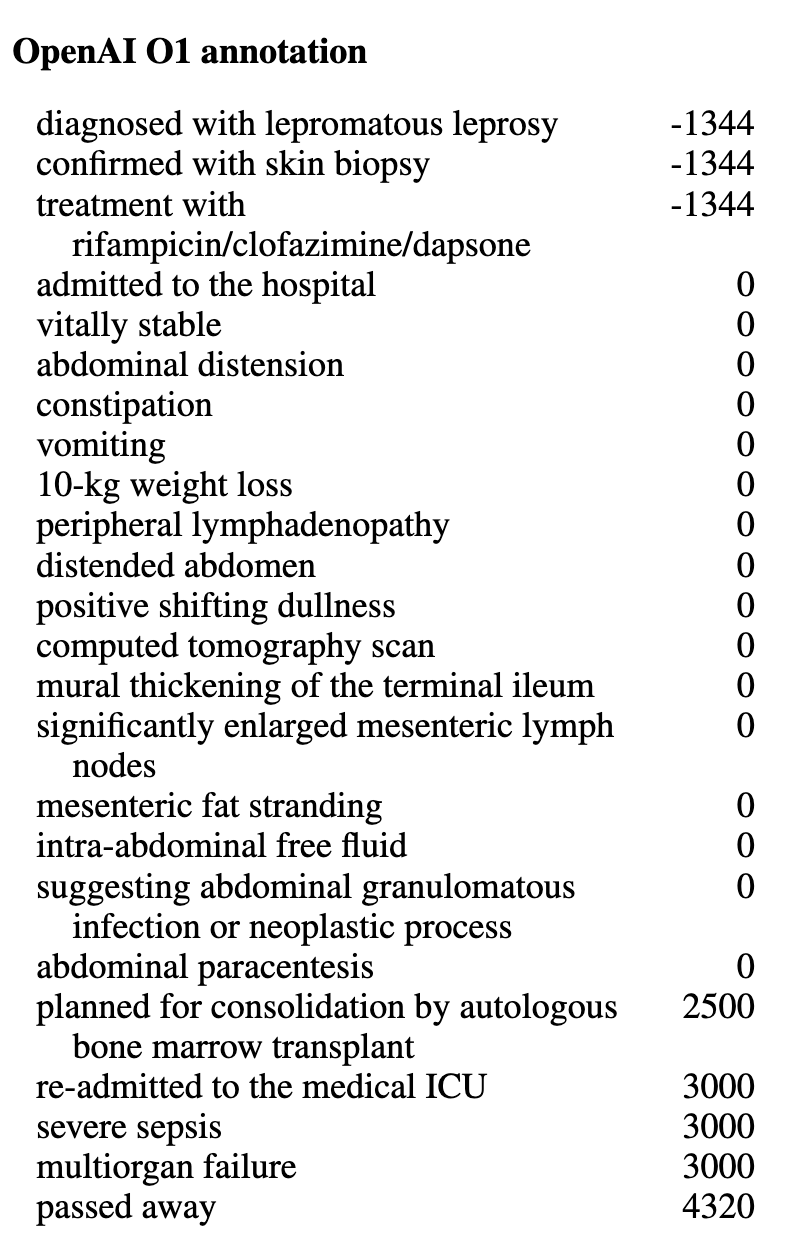
\includegraphics[width=0.95\linewidth]{Scientific_data/Supplementary/example_TTS_for_paper/O1.png}
% \caption*{\texttt{O1}}
% \end{subfigure}

% \vspace{4pt}

% % Row 4
% \begin{subfigure}[t]{0.45\textwidth}
% \centering
% 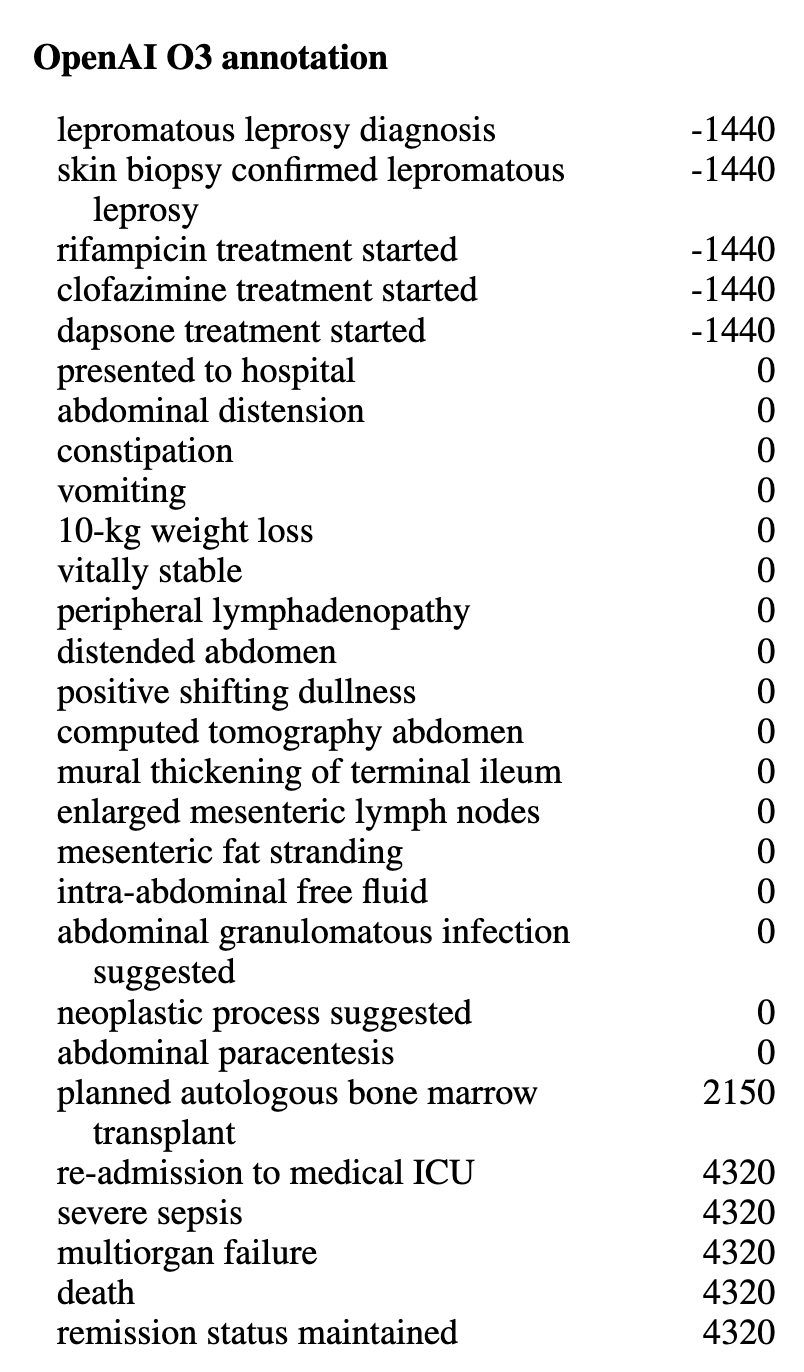
\includegraphics[width=0.95\linewidth]{Scientific_data/Supplementary/example_TTS_for_paper/O3.png}
% \caption*{\texttt{O3}}
% \end{subfigure}
% \hfill
% \begin{subfigure}[t]{0.45\textwidth}
% \centering
% 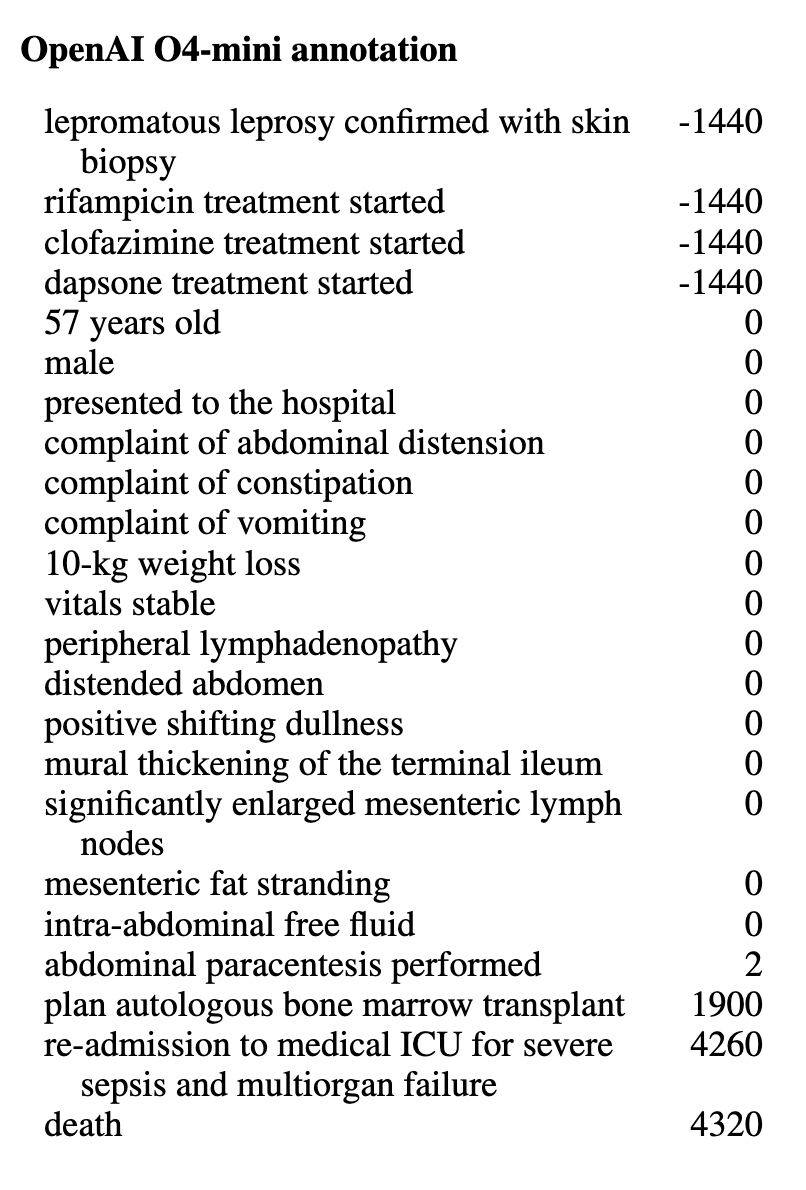
\includegraphics[width=0.95\linewidth]{Scientific_data/Supplementary/example_TTS_for_paper/O4mini.png}
% \caption*{\texttt{O4-mini}}
% \end{subfigure}

% % ---------------------------------------------------
% % Caption + Label
% % ---------------------------------------------------
% \caption{
% Comparison of temporal annotations generated by several LLMs for a representative case report  (PMC10629858). The figure contrasts manual annotations with model-generated event--time sequences, highlighting differences in event granularity, phrasing, duplicate event generation, and  temporal normalization (e.g., variation in converting narrative expressions such as  ``two months before admission'' into hour offsets). Long-range timestamp assignments  (e.g., for transplant planning, ICU readmission, and death) exhibit the greatest variability across models, whereas the overall ordering of major clinical events is largely preserved. 
% This example illustrates characteristic differences in how LLMs interpret, segment, and temporally anchor clinical narratives.
% }
% \label{fig:compare_llm_annotations}

% \vspace{-2mm}
% \end{figure*}


Across annotators, the principal clinical storyline is consistently recovered: antecedent treatment for lepromatous leprosy, hospital presentation with abdominal symptoms and imaging findings, subsequent sepsis with ICU readmission, and death. All models place examination findings and initial presentation at or near the admission anchor ($t{=}0$), assign negative times to pre-admission history, and positive times to later complications, indicating broadly correct temporal polarity and order.

Differences emerge in \textit{event granularity and phrasing}. \texttt{DeepSeek-R1}, \texttt{DeepSeek-V3-0324}, \texttt{LLaMA 3.3 70B}, \texttt{GPT5}, \texttt{O3}, and \texttt{O4-mini} tend to split conjunctions into separate medication events (``rifampicin'', ``clofazimine'', ``dapsone''), whereas \texttt{O1} compresses them into a single treatment line. Near-duplicate entries at the same timestamp (e.g., ``diagnosed with lepromatous leprosy'' and ``skin biopsy confirmed'') appear in \texttt{DeepSeek-R1}, \texttt{DeepSeek-V3-0324}, \texttt{GPT5}, \texttt{O1}, \texttt{O3}, \texttt{O4-mini} (and sometimes \texttt{LLaMA 3.3 70B}). Event specificity also varies: \texttt{DeepSeek-R1}/\texttt{DeepSeek-V3-0324}, \texttt{GPT5}, \texttt{O3}, \texttt{O4-mini}, and \texttt{LLaMA 3.3 70B} more often retain concrete procedures/medications, while \texttt{O1} uses generic descriptors.

We also observe systematic differences in \textit{temporal normalization}. The phrase ``two months before admission'' is mapped to different hour offsets: about $-1464$ by \texttt{DeepSeek-R1} and \texttt{DeepSeek-V3-0324}, $-1440$ by \texttt{GPT5}, \texttt{O3}, and \texttt{O4-mini}, $-1344$ by \texttt{O1}, and $-144$ by \texttt{LLaMA 3.3 70B} (likely a day–hour scaling error). For long-horizon post-admission events, absolute times vary by hundreds of hours across models. The transplant \emph{plan} is placed at $\sim\!672$ h (\texttt{DeepSeek-V3-0324}), $\sim\!1344$ h (\texttt{LLaMA 3.3 70B}), $\sim\!1900$ h (\texttt{O4-mini}), $\sim\!2150$ h (\texttt{O3}), $\sim\!2400$ h (\texttt{GPT5}), $\sim\!2500$ h (\texttt{O1}), and $\sim\!4320$ h (\texttt{DeepSeek-R1}). ICU readmission/sepsis/death also cluster late but with model-specific offsets: $\sim\!4032$ h (\texttt{DeepSeek-V3-0324}), $\sim\!4296$–$4320$ h (\texttt{GPT5}), $\sim\!4260$/$4320$ h (\texttt{O4-mini}), $\sim\!4320$ h (\texttt{O3}, \texttt{DeepSeek-R1}), and $\sim\!3000$ then $4320$ h (\texttt{O1}), whereas \texttt{LLaMA 3.3 70B} assigns earlier times ($\sim\!1344$–$1440$ h). Despite this spread, the relative ordering of major milestones is largely preserved.

A recurrent issue across \emph{all} models is \textit{plan versus action conflation}: statements such as ``planned autologous bone-marrow transplant'' are time-stamped as if they occurred rather than encoded as intent. \textcolor{red}{Jeremy: To clarify, the timestamping of the schedule time for this is fine (it is timestampable and could affect health risk via anticipatory decision-making).  But if the word "planned" is omitted, then it is encoded as occurred rather than intent. So it would be the event string (not the timestamp) that is problematic in this case.} 
Overall, the models capture the sequence of key events but differ in how they segment conjunctive statements (\texttt{O1} compressed vs.\ others split), handle near-duplicates, and resolve absolute times (month-to-hour mapping and long-range offsets). Although a single case cannot support definitive conclusions, these qualitative trends were observed repeatedly across additional case reports and are consistent with the aggregate metrics in Section 5.2.


%%%%%%%%%%%%%%%%%%%%%%%%%%%%%%%%%%%%%
%%%%%%%%%%%%%%%%%%%%%%%%%%%%%%%%%%%%%

\subsection{Limitations and future directions}

Our temporal annotation pipeline has some important caveats to consider. First, the pipeline relies on case reports from the PubMed Open Access (PMOA) corpus, which often reflect rare or atypical presentations and differ from routine clinical notes (e.g., progress notes, discharge summaries in MIMIC III/IV), potentially limiting the model’s generalizability to real-world health system texts. Compared to routine clinical notes, case reports offer rich, temporally structured narratives with explicit clinical rationale, making them especially useful for evaluating model performance under sparse documentation. Our LLM-assisted pipeline is a generalized framework for temporal annotations of clinical narratives using PubMed case reports as a benchmark with scope of future applications on MIMIC IV discharge summaries.  

Second, we model events as minimally modified text spans to preserve alignment with the source text, which facilitates interpretability but relies heavily on embedding-based comparison and forgoes normalization to standard clinical ontologies like UMLS.

Third, representing time with single relative points simplifies annotation but limits expressiveness, especially in cases where durations or implicit temporal relationships are critical. 

Fourth, our one-to-one recursive event matching strategy prioritizes temporal consistency, but at the cost of reduced recall, particularly when events are expressed as conjunctive or split mentions. These design choices emphasize precision and contextual grounding but leave room for enhancements in coverage and temporal fidelity. Future work could incorporate LLM ensembling, prompt engineering, or active learning-based fine-tuning to further improve event-time extraction.

Finally, the manual reference set comprises 200 cases annotated by a single clinical expert; as a result, we cannot estimate inter-annotator agreement, and evaluation metrics reflect agreement with that expert rather than adjudicated consensus.
